\documentclass{beamer}
\usetheme{Madrid}

\usepackage[utf8]{inputenc} % solo si usas pdflatex
\usepackage[T1]{fontenc}    % solo si usas pdflatex

\usepackage{amsmath,amssymb}
\usepackage{microtype}
\usepackage{cancel}         % si lo usas
\usepackage{fontawesome}    % si lo usas
% \usepackage{xypic}        % solo si lo usas
% \usepackage{multicol}     % normalmente no; usar columns de beamer
% \usepackage{amsthm}       % solo si defines teoremas propios
% \usepackage{scrextend}    % solo si lo usas

\usepackage{graphicx}
\graphicspath{{images/}}

\hypersetup{pdfborder={0 0 0}}


\title{Seguridad de la Información}
\author{Rodrigo Blanco Betes. Alfa Formación}
\date{Enero del 2026}

\begin{document}

\begin{frame}
\titlepage
\end{frame}

\begin{frame}
\tableofcontents
\end{frame}

%-------------------------------------------------

\section{Fundamentos de la seguridad de la información}

\begin{frame}{Seguridad de la información}
\begin{itemize}
    \item Protege la información frente a accesos no autorizados.
    \item Evita modificaciones indebidas de los datos.
    \item Reduce pérdidas de información.
    \item Garantiza la continuidad del servicio.
\end{itemize}
\end{frame}

\begin{frame}{Seguridad vs fiabilidad}
\begin{itemize}
    \item La fiabilidad mide si un sistema funciona correctamente en el tiempo.
    \item Un sistema seguro pero no fiable resulta inútil.
    \item La seguridad no sustituye a la fiabilidad.
    \item Ambos conceptos deben coexistir.
\end{itemize}
\end{frame}

\begin{frame}{Objetivo de los sistemas informáticos}
\begin{itemize}
    \item Funcionamiento correcto y predecible.
    \item Protección de la información.
    \item Disponibilidad continua del servicio.
    \item Seguridad integrada desde el diseño.
\end{itemize}
\end{frame}

%-------------------------------------------------

\section{Las bases de la seguridad: CIA y AAA}

\begin{frame}{La tríada CIA}
\begin{itemize}
    \item Modelo fundamental de la seguridad de la información.
    \item Se compone de tres principios clave.
    \item Cubre acceso, modificación y disponibilidad de la información.
\end{itemize}
\end{frame}

\begin{frame}{Confidencialidad}
\begin{itemize}
    \item Solo acceden usuarios autorizados.
    \item Se apoya en el cifrado de datos.
    \item Utiliza controles de acceso.
    \item Requiere autenticación de usuarios.
\end{itemize}
\end{frame}

\begin{frame}{Integridad}
\begin{itemize}
    \item Garantiza que la información no ha sido alterada.
    \item Detecta modificaciones no autorizadas.
    \item Se basa en funciones hash.
    \item Usa firmas digitales y control de versiones.
\end{itemize}
\end{frame}

\begin{frame}{Disponibilidad}
\begin{itemize}
    \item La información debe estar accesible cuando se necesita.
    \item Se apoya en copias de seguridad.
    \item Utiliza sistemas redundantes.
    \item Protege frente a ataques DoS.
\end{itemize}
\end{frame}

\begin{frame}{Modelo AAA}
\begin{itemize}
    \item Autenticación: verifica la identidad del usuario.
    \item Autorización: define qué acciones puede realizar.
    \item Auditoría: registra actividades y responsabilidades.
\end{itemize}
\end{frame}

\begin{frame}{Mecanismos de seguridad}
\begin{itemize}
    \item Previenen, detectan y mitigan riesgos.
    \item Incluyen firewalls y sistemas de detección de intrusos.
    \item Usan cifrado y copias de seguridad.
    \item Funcionan mejor por capas y redundancia.
\end{itemize}
\end{frame}

%-------------------------------------------------

\section{Vulnerabilidades y amenazas}

\begin{frame}{Vulnerabilidades}
\begin{itemize}
    \item Son debilidades del sistema.
    \item Pueden existir en software, procesos o configuraciones.
    \item Surgen por falta de actualizaciones.
    \item Se agravan con contraseñas débiles o permisos mal asignados.
\end{itemize}
\end{frame}

\begin{frame}{Amenazas}
\begin{itemize}
    \item Son eventos potencialmente dañinos.
    \item Explotan vulnerabilidades existentes.
    \item Pueden ser humanas o técnicas.
    \item Incluyen errores y ataques intencionados.
\end{itemize}
\end{frame}

\begin{frame}{Ataques}
\begin{itemize}
    \item Son la materialización de una amenaza.
    \item Ocurren cuando se explota una vulnerabilidad.
    \item Pueden causar pérdida de datos o servicio.
\end{itemize}
\end{frame}

\begin{frame}{Clasificación de amenazas}
\begin{itemize}
    \item Internas: usuarios con acceso legítimo.
    \item Externas: atacantes, bots u organizaciones criminales.
    \item Accidentales: errores humanos o fallos técnicos.
    \item Intencionadas: ataques planificados.
\end{itemize}
\end{frame}

\begin{frame}{Tipos de amenazas}
\begin{itemize}
    \item Malware: virus, troyanos y ransomware.
    \item Ingeniería social y phishing.
    \item Ataques de red como DoS o MITM.
\end{itemize}
\end{frame}

%-------------------------------------------------

\section{Criptografía básica}

\begin{frame}{¿Qué es la criptografía?}
\begin{itemize}
  \item La criptografía protege la información mediante técnicas matemáticas y algoritmos.
  \item Permite que los datos solo sean entendidos por las partes autorizadas.
  \item Evita que terceros puedan:
  \begin{itemize}
    \item Leer
    \item Modificar
    \item Falsificar la información
  \end{itemize}
\end{itemize}
\end{frame}

\begin{frame}{Objetivos de la criptografía}
\begin{itemize}
  \item Confidencialidad: impide accesos no autorizados.
  \item Integridad: permite detectar modificaciones en la información.
  \item Autenticación: verifica la identidad de las partes que se comunican.
\end{itemize}
\end{frame}

\begin{frame}{Conceptos básicos}
\begin{itemize}
  \item \textbf{Texto en claro}: información legible.
  \item \textbf{Texto cifrado}: información ilegible.
  \item \textbf{Cifrado}: proceso de transformación del texto en claro.
  \item \textbf{Clave criptográfica}: valor secreto necesario para descifrar.
\end{itemize}
\end{frame}

\begin{frame}{Tipos de criptografía}
\begin{itemize}
  \item \textbf{Criptografía simétrica}
  \begin{itemize}
    \item Una única clave para cifrar y descifrar
    \item Rápida, pero requiere compartir la clave de forma segura
  \end{itemize}
  \item \textbf{Criptografía asimétrica}
  \begin{itemize}
    \item Par de claves: pública y privada
    \item No requiere intercambio previo de claves secretas
  \end{itemize}
\end{itemize}
\end{frame}

\begin{frame}{Funciones hash}
\begin{itemize}
  \item No cifran información.
  \item Generan un resumen único de los datos.
  \item Permiten verificar la integridad de la información.
\end{itemize}
\end{frame}

\begin{frame}{Criptografía en la vida diaria}
\begin{itemize}
  \item Navegación web segura (HTTPS)
  \item Almacenamiento de contraseñas
  \item Firmas digitales
  \item Comunicaciones cifradas
  \item Autenticación y control de acceso
\end{itemize}
\end{frame}

\subsection{Formas de cifrado habituales}

\begin{frame}{AES (Advanced Encryption Standard)}
\begin{itemize}
  \item Cifrado simétrico más utilizado actualmente.
  \item Diseñado por Vincent Rijmen y Joan Daemen (1998).
  \item Recomendado por organismos como el NIST.
  \item Usado en discos cifrados y comunicaciones seguras.
\end{itemize}
\end{frame}

\begin{frame}{Características de AES}
\begin{itemize}
  \item Misma clave para cifrar y descifrar.
  \item Seguridad basada en mantener la clave secreta.
  \item Tamaño de bloque fijo: \textbf{128 bits}.
  \item Tamaños de clave:
  \begin{itemize}
    \item 128 bits
    \item 192 bits
    \item 256 bits
  \end{itemize}
\end{itemize}
\end{frame}

\begin{frame}{Fases del cifrado AES}
\begin{enumerate}
  \item SubBytes
  \item ShiftRows
  \item MixColumns
  \item AddRoundKey
\end{enumerate}
\end{frame}

\begin{frame}{AES – Fase SubBytes}
\begin{itemize}
  \item Sustitución no lineal de cada byte.
  \item Bloques organizados en una matriz $4 \times 4$.
  \item Dificulta ataques basados en patrones.
\end{itemize}
\begin{center}
  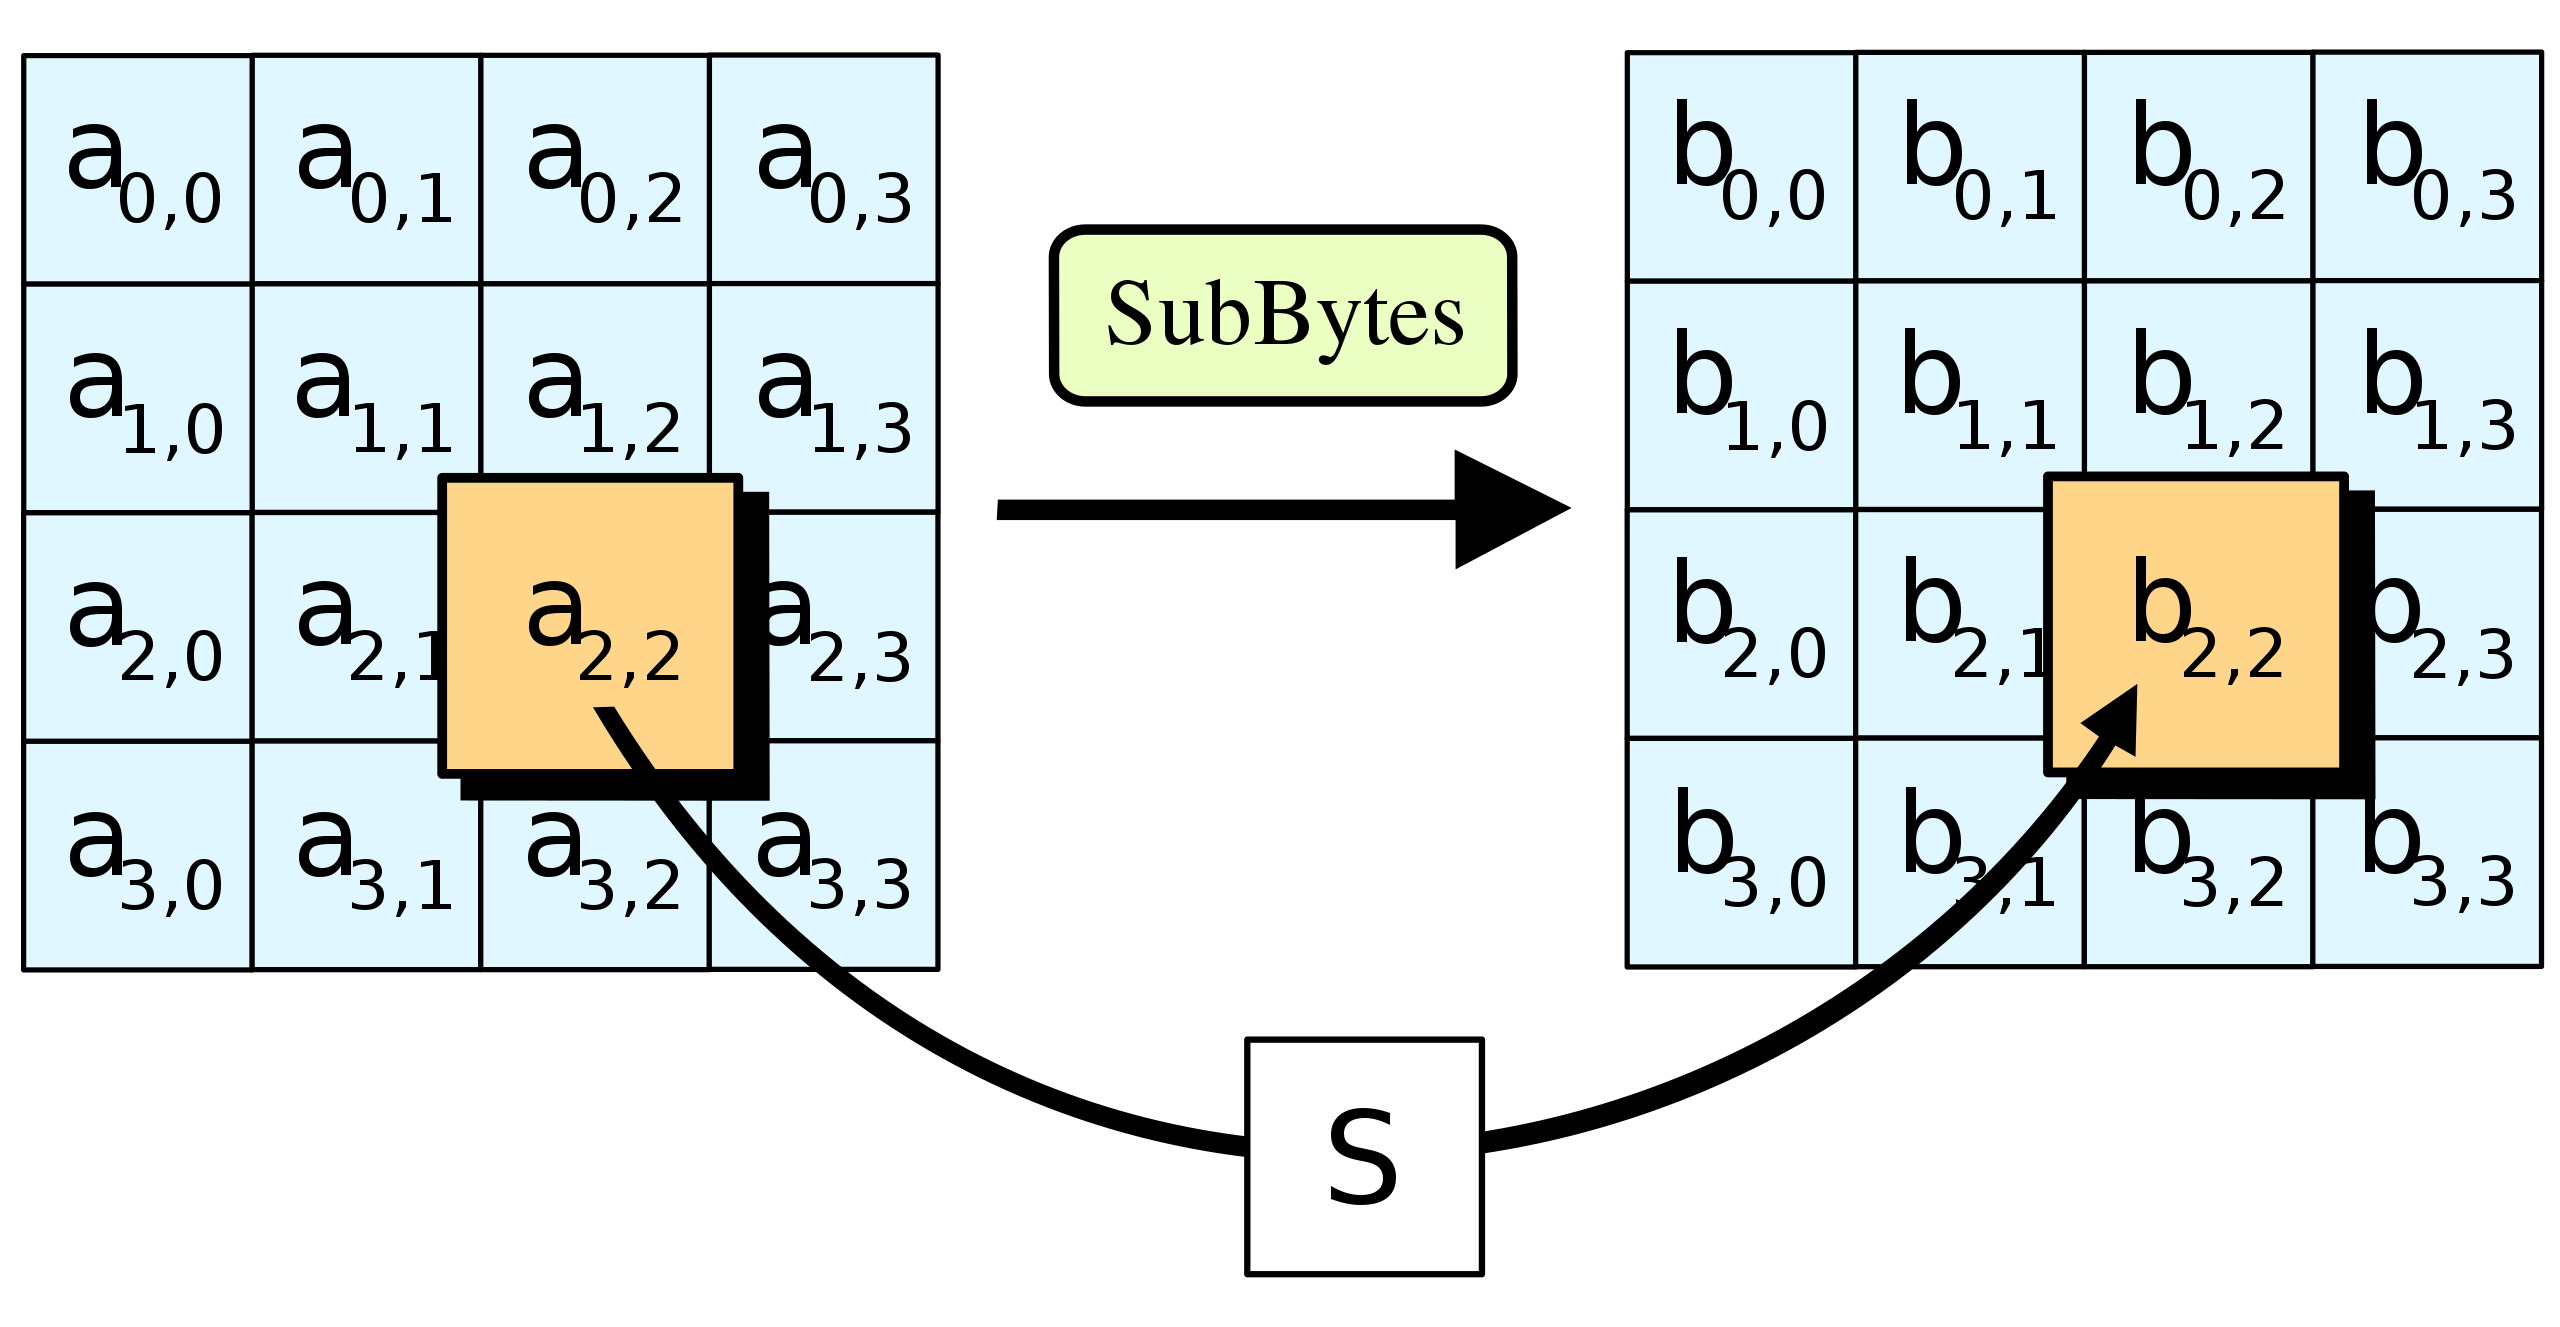
\includegraphics[width=0.5\textwidth]{2560px-AES-SubBytes.svg.png}
\end{center}
\end{frame}

\begin{frame}{AES – Fase ShiftRows}
\begin{itemize}
  \item Rotación de filas del bloque.
  \item Cada fila se desplaza un número distinto de posiciones.
\end{itemize}
\begin{center}
  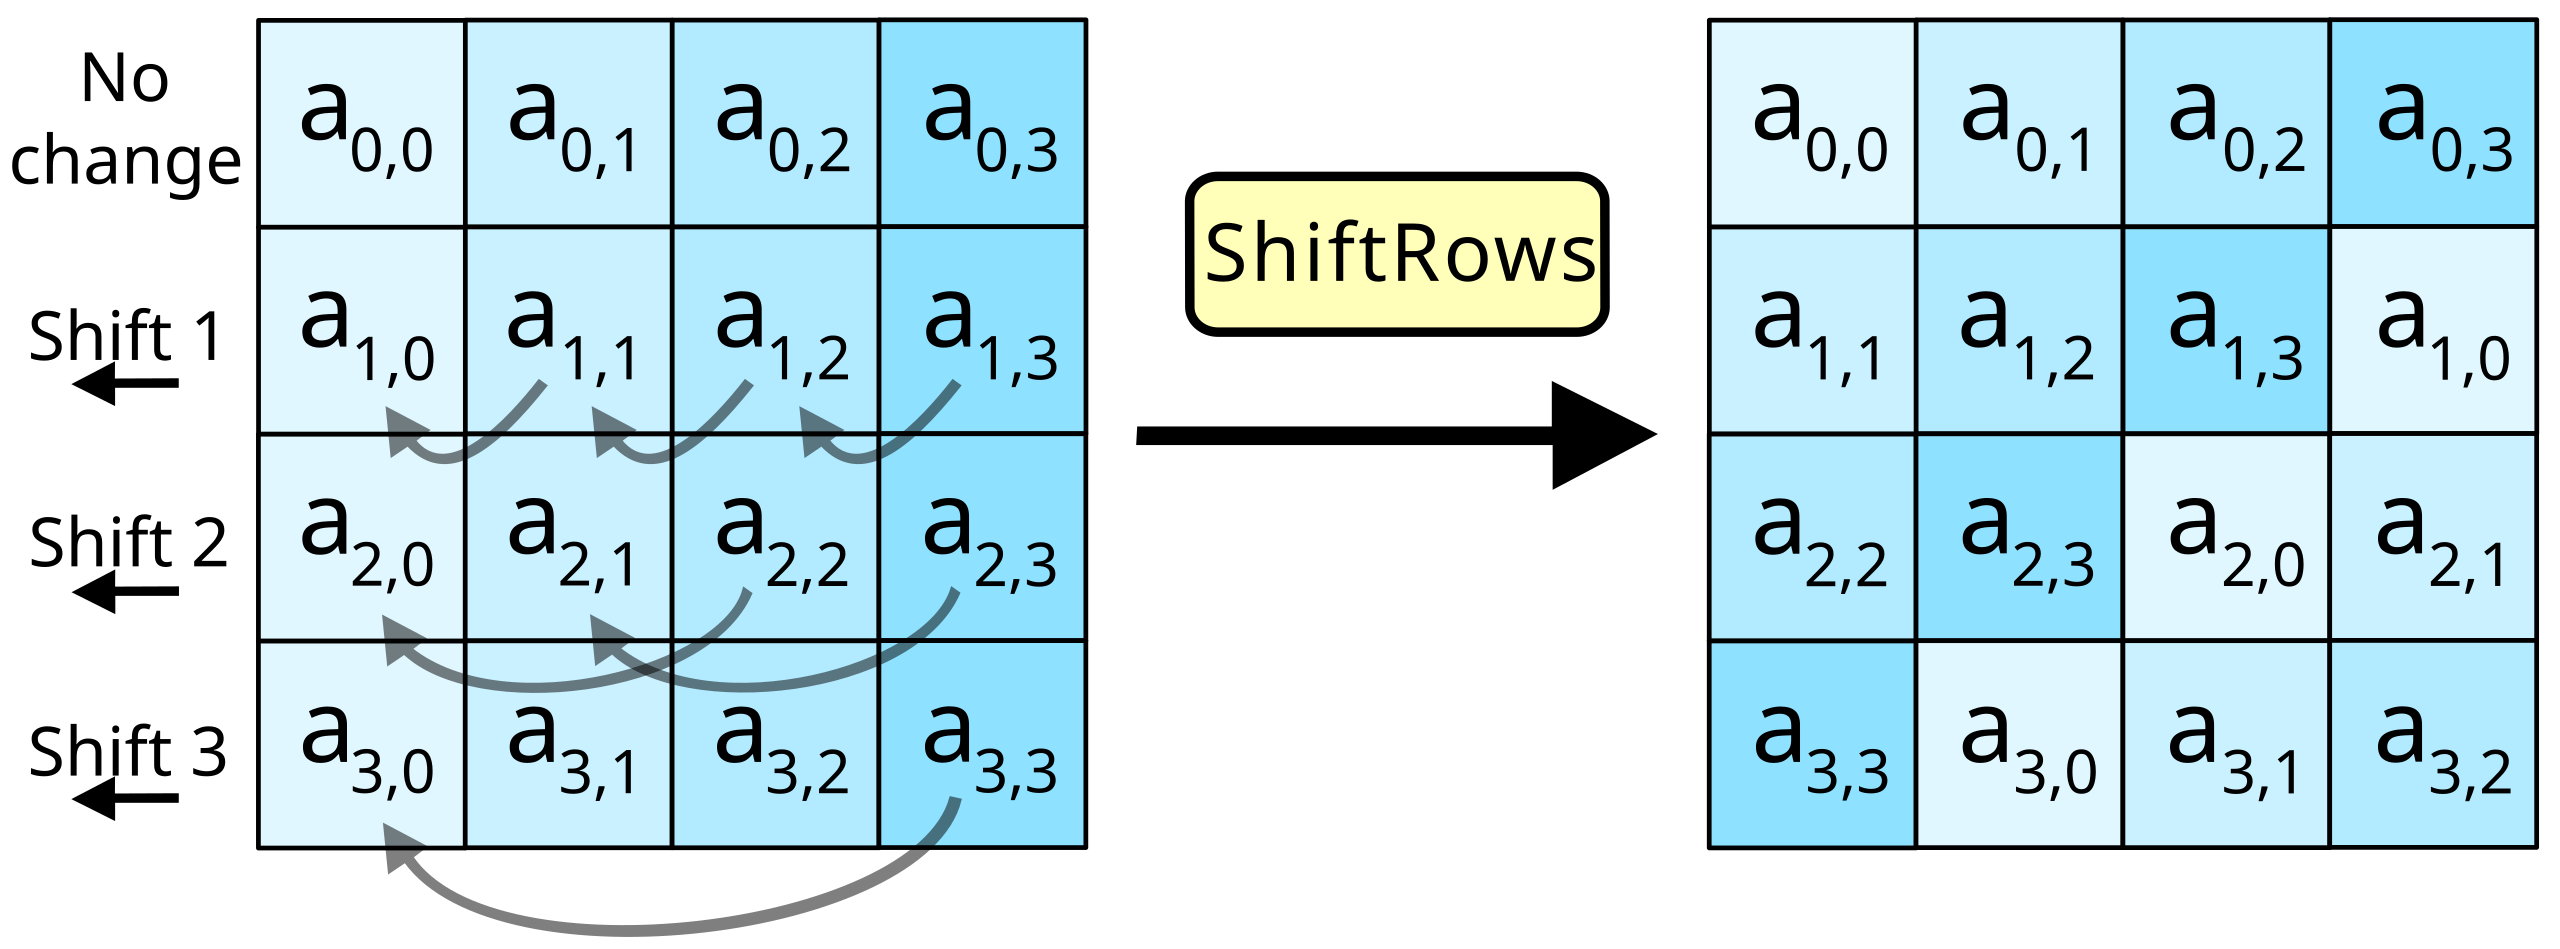
\includegraphics[width=0.5\linewidth]{ShiftRows.png}
\end{center}
\end{frame}

\begin{frame}{AES – Fase MixColumns}
\begin{itemize}
  \item Transformación lineal invertible de cada bloque.
  \item Uso de coeficientes fijos para mezclar los datos.
\end{itemize}
\begin{center}
  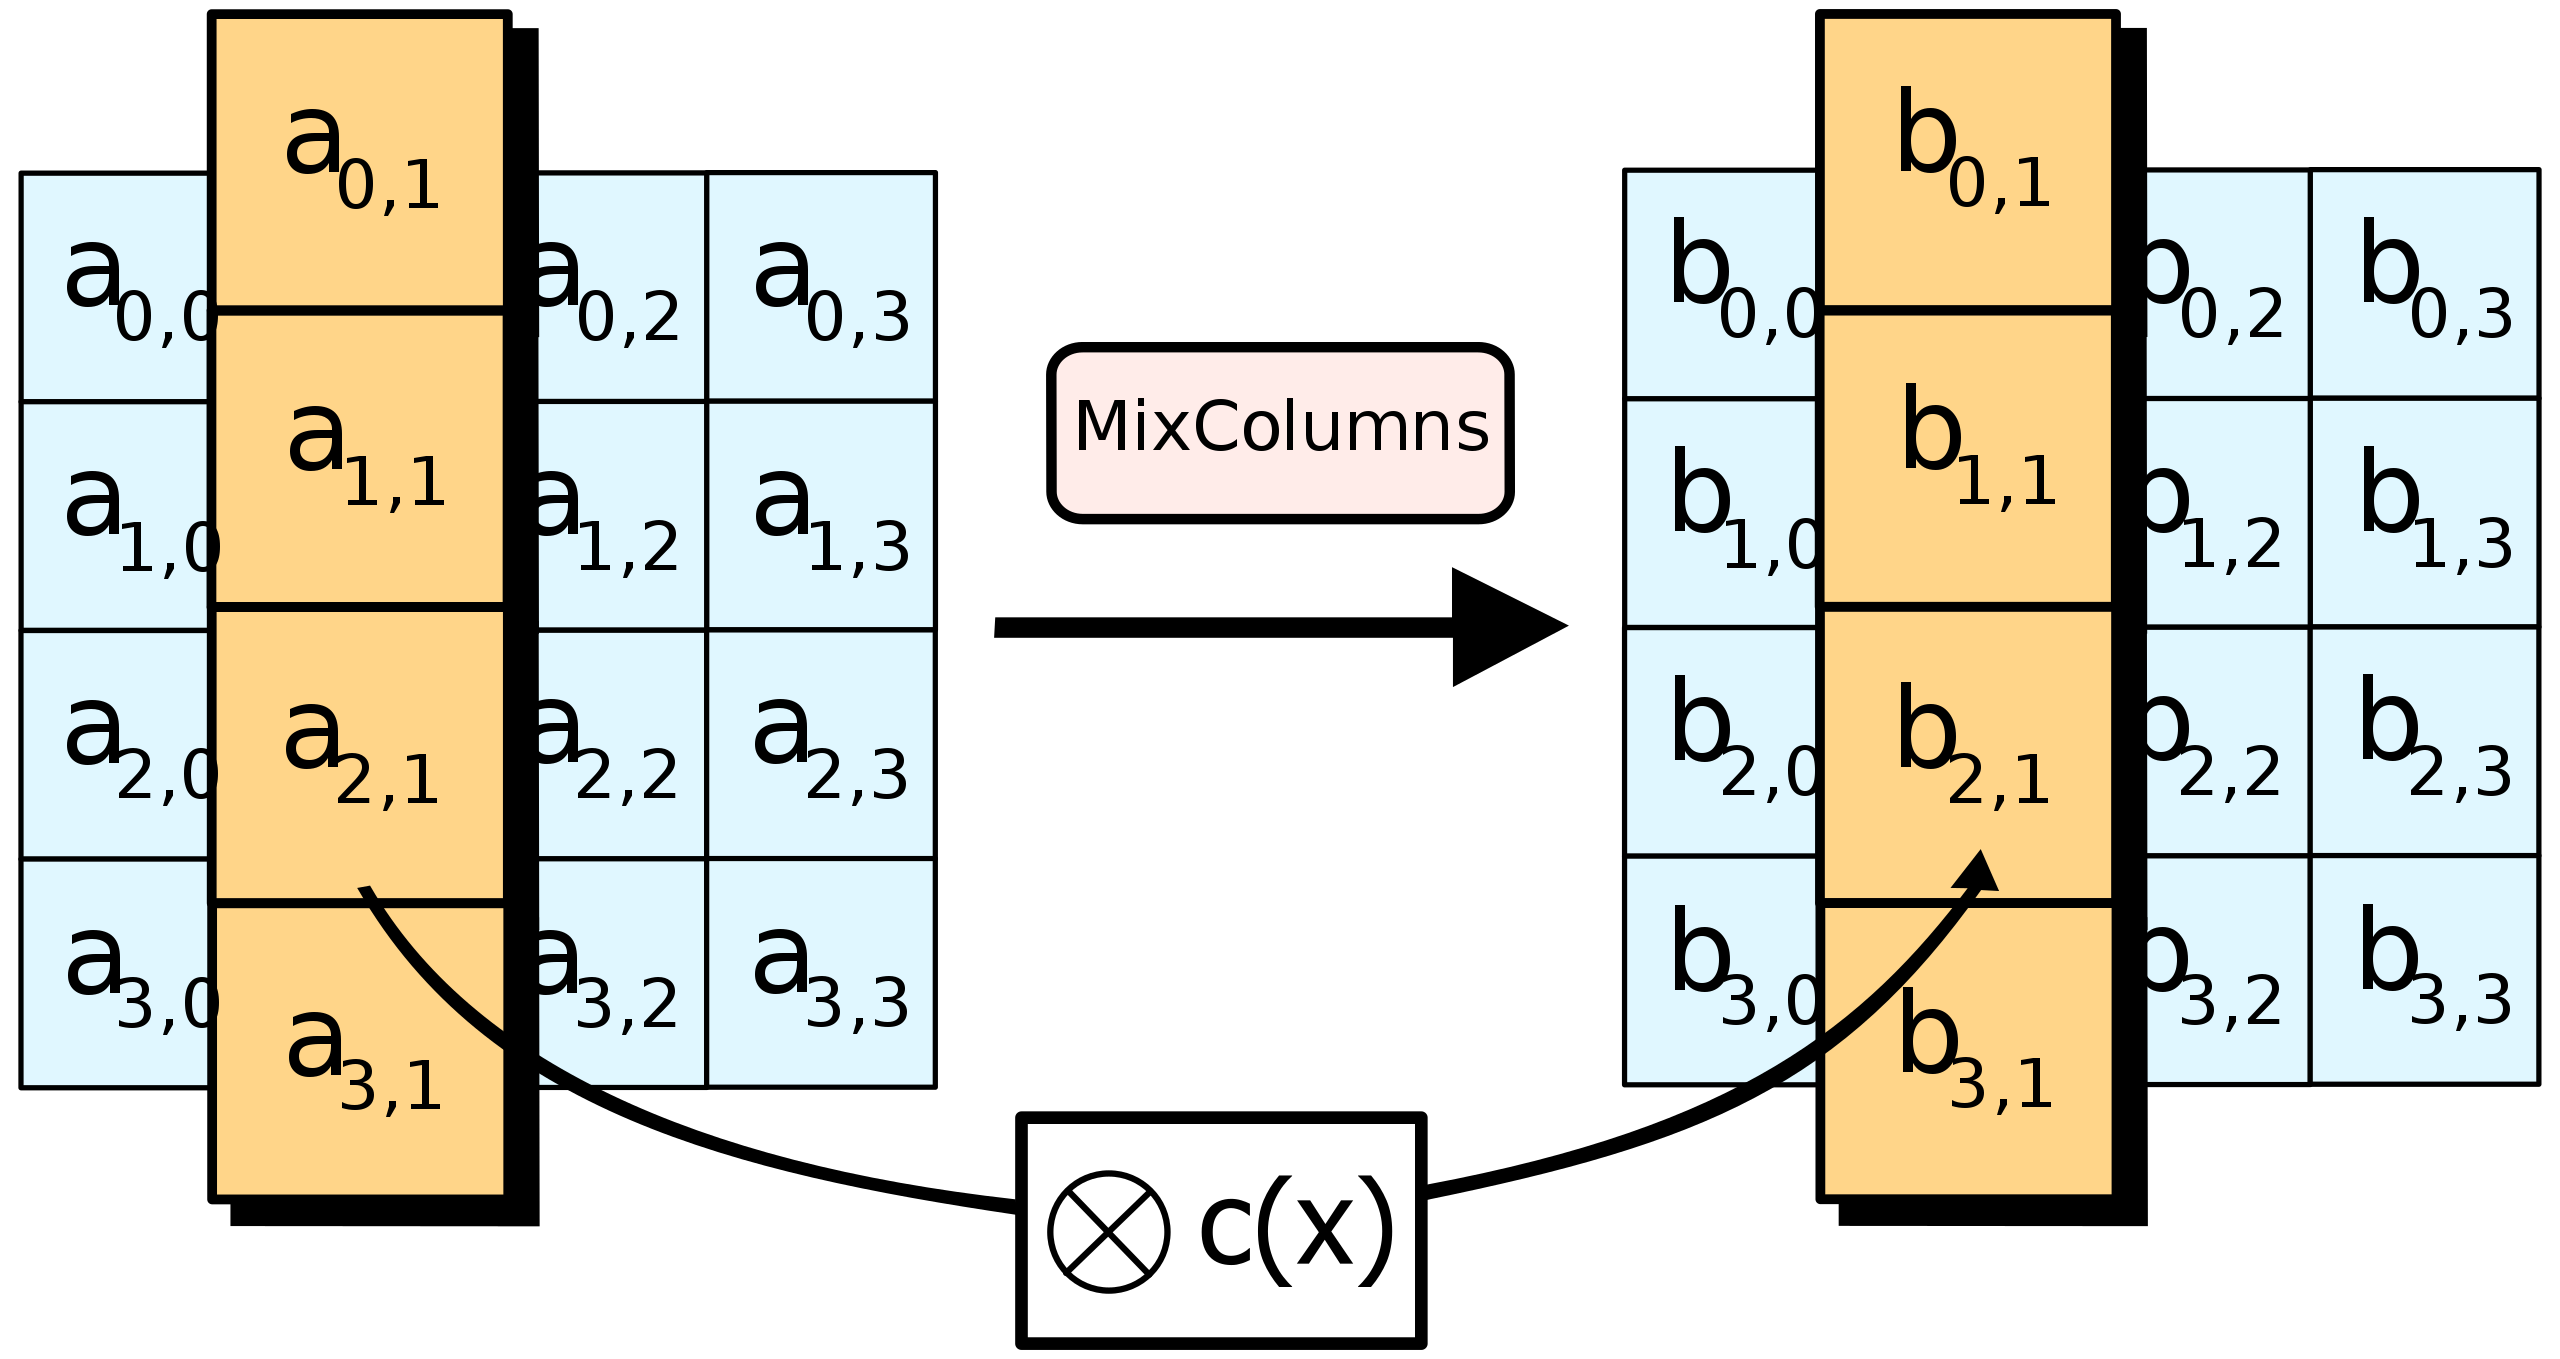
\includegraphics[width=0.5\linewidth]{MixColumns.png}
\end{center}
\end{frame}

\begin{frame}{AES – Fase AddRoundKey}
\begin{itemize}
  \item Única fase donde se usa la clave secreta.
  \item Operación XOR entre el bloque y la subclave.
  \item Se aplica en cada ronda de cifrado.
\end{itemize}
\begin{center}
  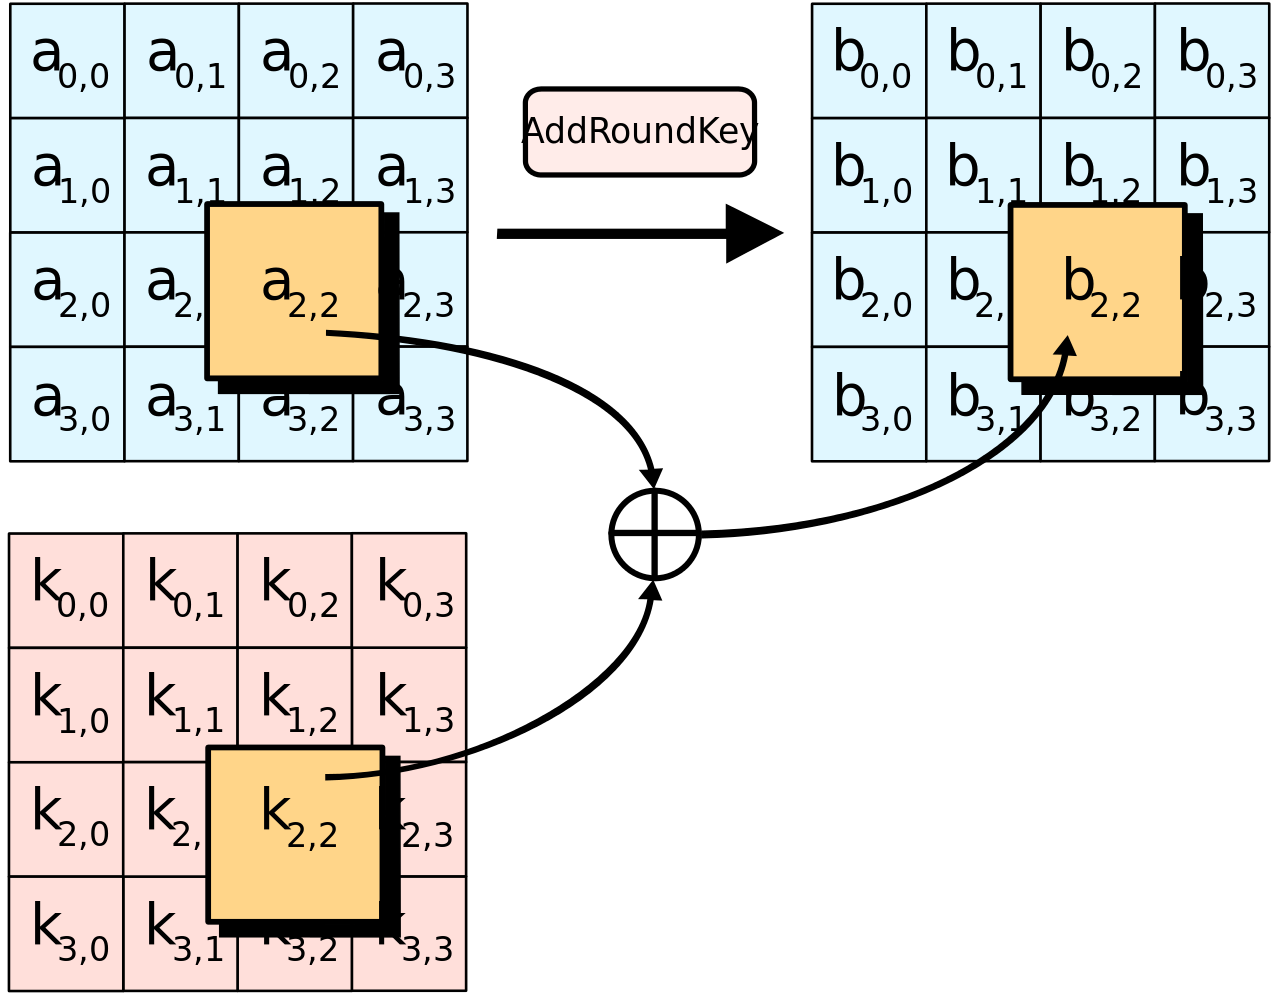
\includegraphics[width=0.5\linewidth]{AddRoundKey.png}
\end{center}
\end{frame}

\begin{frame}{Rondas de cifrado en AES}
\begin{itemize}
  \item Las cuatro fases se repiten en múltiples rondas.
  \item Aumentan significativamente la seguridad.
  \item Las claves largas se dividen en subclaves.
\end{itemize}
\end{frame}

\begin{frame}{Usos habituales de AES (I)}
\begin{itemize}
  \item Comunicaciones seguras en Internet (HTTPS, TLS).
  \item Cifrado de discos y almacenamiento:
  \begin{itemize}
    \item BitLocker
    \item FileVault
    \item LUKS
  \end{itemize}
  \item Cifrado de archivos y carpetas.
\end{itemize}
\end{frame}

\begin{frame}{Usos habituales de AES (II)}
\begin{itemize}
  \item Redes privadas virtuales (VPN):
  \begin{itemize}
    \item OpenVPN
    \item IPsec
    \item WireGuard
  \end{itemize}
  \item Bases de datos y cifrado de datos en reposo.
  \item Servicios en la nube (AWS, Azure, GCP).
\end{itemize}
\end{frame}

\begin{frame}{Usos habituales de AES (III)}
\begin{itemize}
  \item Hardware y sistemas embebidos:
  \begin{itemize}
    \item TPM
    \item HSM
    \item IoT
  \end{itemize}
  \item Protección de almacenes de secretos.
  \item Contraseñas protegidas mediante funciones hash.
\end{itemize}
\end{frame}

%-------------------------------------

\begin{frame}{RSA: introducción}
\begin{itemize}
  \item Uno de los sistemas de cifrado asimétrico más influyentes.
  \item Propuesto en 1977 por:
  \begin{itemize}
    \item Ronald Rivest
    \item Adi Shamir
    \item Leonard Adleman
  \end{itemize}
  \item Su nombre proviene de las iniciales de sus creadores.
\end{itemize}
\end{frame}

\begin{frame}{Claves en RSA}
\begin{itemize}
  \item RSA es un cifrado \textbf{asimétrico}.
  \item Utiliza dos claves:
  \begin{itemize}
    \item \textbf{Clave pública} $e$
    \item \textbf{Clave privada} $d$
  \end{itemize}
  \item La clave pública permite cifrar mensajes.
  \item Solo el receptor puede descifrarlos con la clave privada.
\end{itemize}
\end{frame}

\begin{frame}{Funcionamiento matemático de RSA}
\begin{itemize}
  \item El mensaje $M$ se representa como un número entero.
  \item Cifrado:
  \[
    c \equiv M^e \; (\text{mod } n)
  \]
  \item Descifrado:
  \[
    M \equiv c^d \; (\text{mod } n)
  \]
  \item Las claves cumplen:
  \[
    e \cdot d \equiv 1 \; (\text{mod } n)
  \]
\end{itemize}
\end{frame}

\begin{frame}{Fundamento de seguridad de RSA}
\begin{itemize}
  \item La seguridad se basa en la dificultad de:
  \begin{itemize}
    \item Factorizar un número $n = p \cdot q$
    \item Donde $p$ y $q$ son primos muy grandes
  \end{itemize}
  \item Actualmente no existe un algoritmo clásico eficiente para este problema.
  \item A partir de $n$ se derivan las claves pública y privada.
\end{itemize}
\end{frame}

\begin{frame}{RSA y computación cuántica}
\begin{itemize}
  \item La computación cuántica amenaza la seguridad de RSA.
  \item El \textbf{algoritmo de Shor} permite factorizar $n$ en tiempo razonable.
  \item Actualmente el tamaño de los ordenadores cuánticos es limitado.
  \item Si esta tecnología avanza, RSA quedaría comprometido.
  \item Este problema no afecta a sistemas simétricos como AES.
\end{itemize}
\end{frame}

\begin{frame}{Usos principales de RSA}
\begin{itemize}
  \item No se usa para cifrar grandes volúmenes de datos.
  \item Se emplea principalmente para:
  \begin{itemize}
    \item Intercambio seguro de claves
    \item Autenticación
  \end{itemize}
  \item Suele cifrar claves simétricas (por ejemplo, AES).
\end{itemize}
\end{frame}

\begin{frame}{Aplicaciones habituales de RSA}
\begin{itemize}
  \item Certificados digitales y autenticación de servidores web.
  \item Firmas digitales:
  \begin{itemize}
    \item Se firma un hash con la clave privada
    \item Se verifica con la clave pública
  \end{itemize}
  \item Sistemas heredados por compatibilidad.
  \item No es adecuado para datos en reposo:
  \begin{itemize}
    \item Costoso
    \item Poco escalable
  \end{itemize}
\end{itemize}
\end{frame}

%-----------------------------------------


\begin{frame}{Cifrado de curvas elípticas (ECC)}
\begin{itemize}
  \item Sistema de criptografía de clave pública.
  \item Basado en propiedades algebraicas de curvas elípticas.
  \item Definido sobre cuerpos finitos.
  \item Su seguridad se basa en el problema del logaritmo discreto.
\end{itemize}
\end{frame}

\begin{frame}{Curvas elípticas}
\begin{itemize}
  \item Se describen mediante ecuaciones del tipo:
  \[
    y^2 = x^3 + ax + b
  \]
  \item $a$ y $b$ determinan la forma de la curva.
  \item Las operaciones se realizan módulo $p$, con $p$ primo.
\end{itemize}
\end{frame}

\begin{frame}{ECC frente a otros sistemas}
\begin{itemize}
  \item ECC ofrece operaciones de:
  \begin{itemize}
    \item Clave pública
    \item Firma digital
  \end{itemize}
  \item Es más eficiente que sistemas tradicionales como RSA.
\end{itemize}
\end{frame}

\begin{frame}{Ventajas de ECC}
\begin{itemize}
  \item \textbf{Mayor seguridad con claves más pequeñas}
  \begin{itemize}
    \item 256 bits en ECC $\approx$ 3072 bits en RSA
  \end{itemize}
  \item Ideal para dispositivos con recursos limitados.
\end{itemize}
\end{frame}

\begin{frame}{Ventajas de ECC (II)}
\begin{itemize}
  \item \textbf{Eficiencia computacional}
  \begin{itemize}
    \item Menor consumo de CPU
    \item Operaciones más rápidas
  \end{itemize}
  \item \textbf{Uso eficiente de ancho de banda}
  \item \textbf{Seguridad a largo plazo}
\end{itemize}
\end{frame}

\begin{frame}{Aplicaciones de ECC}
\begin{itemize}
  \item Firmas digitales (ECDSA).
  \item Intercambio seguro de claves (ECDH).
  \item Protocolos de seguridad:
  \begin{itemize}
    \item TLS
    \item SSL
  \end{itemize}
\end{itemize}
\end{frame}

\begin{frame}{ECC en sistemas modernos}
\begin{itemize}
  \item Dispositivos móviles y entornos IoT.
  \item Comunicaciones seguras con recursos limitados.
  \item Criptomonedas:
  \begin{itemize}
    \item Bitcoin
    \item Protección de claves privadas
  \end{itemize}
\end{itemize}
\end{frame}

\begin{frame}{Conclusión}
\begin{itemize}
  \item ECC ofrece alta seguridad con claves pequeñas.
  \item Es eficiente y escalable.
  \item Se ha convertido en una pieza clave de la criptografía moderna.
\end{itemize}
\end{frame}

%----------------------------------------------------------

\subsection{Funciones hash}
\label{hash}

\begin{frame}{¿Qué es una función hash?}
\begin{itemize}
  \item Una \textbf{función hash} transforma un dato de entrada de tamaño variable
  \item Produce una \textbf{cadena de longitud fija}
  \item El resultado se denomina \textbf{hash} o resumen
  \item La entrada puede ser:
  \begin{itemize}
    \item Texto
    \item Archivos
    \item Números
    \end{itemize}
\end{itemize}
\end{frame}

\begin{frame}{Propiedades de una función hash}
\begin{enumerate}
  \item Determinista
  \item Salida de tamaño fijo
  \item Rápida de calcular
  \item Unidireccional
  \item Sensible a cambios
  \item Baja probabilidad de colisiones
\end{enumerate}
\end{frame}

\begin{frame}{Propiedades clave (detalle)}
\begin{itemize}
  \item \textbf{Unidireccionalidad}:
  \begin{itemize}
    \item No es viable recuperar la entrada original a partir del hash
  \end{itemize}
  \item \textbf{Sensibilidad a cambios}:
  \begin{itemize}
    \item Un pequeño cambio genera un hash completamente distinto
  \end{itemize}
  \item \textbf{Colisiones}:
  \begin{itemize}
    \item Dos entradas distintas no deberían producir el mismo hash
  \end{itemize}
\end{itemize}
\end{frame}

\begin{frame}{Ejemplo de función hash}
\begin{itemize}
  \item Entrada:
  \begin{center}
    \texttt{"hola"}
  \end{center}
  \item Salida (SHA-256):
  \begin{center}
    \tiny
    \texttt{b94d27b9934d3e08a52e52d7da7dabfac484efe37a5380ee9088f7ace2efcde9}
  \end{center}
\end{itemize}
\end{frame}

\begin{frame}{Sensibilidad a cambios}
\begin{itemize}
  \item Entrada:
  \begin{center}
    \texttt{"Hola"}
  \end{center}
  \item Salida (SHA-256):
  \begin{center}
    \tiny
    \texttt{e633f4fc79e4d91c5d66f1b3e6c2c8a6b87a0c7e9c51eaa9a6fbe65e0bce5f3a}
  \end{center}
  \item Un cambio mínimo genera un hash totalmente distinto
\end{itemize}
\end{frame}

\begin{frame}{Usos de las funciones hash}
\begin{itemize}
  \item Las funciones hash se usan ampliamente en la práctica
  \item Aparecen en:
  \begin{itemize}
    \item Seguridad
    \item Estructuras de datos
    \item Verificación de información
  \end{itemize}
\end{itemize}
\end{frame}

\begin{frame}{Almacenamiento seguro de contraseñas}
\begin{itemize}
  \item No se almacenan contraseñas en claro
  \item Se almacena el \textbf{hash} de la contraseña
  \item Al iniciar sesión:
  \begin{itemize}
    \item Se calcula el hash de la contraseña introducida
    \item Se compara con el hash almacenado
  \end{itemize}
  \item Aunque se robe la base de datos, las contraseñas no quedan expuestas
\end{itemize}
\end{frame}

\begin{frame}{Estructuras de datos: tablas hash}
\begin{itemize}
  \item Uso en diccionarios, mapas y conjuntos
  \item Permiten búsquedas muy eficientes
  \item Coste constante en la práctica: $O(1)$
  \item Muy utilizadas en lenguajes de programación
\end{itemize}
\end{frame}

\begin{frame}{Verificación de integridad de archivos}
\begin{itemize}
  \item Al descargar archivos se proporciona un hash
  \item Ejemplo:
  \begin{center}
    \texttt{SHA-256: a3f5c8e9...}
  \end{center}
  \item Se compara el hash del archivo descargado
  \item Si coinciden, el archivo no ha sido alterado
\end{itemize}
\end{frame}

\begin{frame}{Firmas digitales y blockchain}
\begin{itemize}
  \item En blockchain:
  \begin{itemize}
    \item Cada bloque contiene el hash del bloque anterior
    \item Alterar un bloque rompe toda la cadena
  \end{itemize}
  \item Garantiza:
  \begin{itemize}
    \item Integridad
    \item Inmutabilidad
  \end{itemize}
\end{itemize}
\end{frame}

\begin{frame}{Otros usos de funciones hash}
\begin{itemize}
  \item Detección de archivos duplicados
  \item Indexación de grandes volúmenes de datos
  \item Sistemas de caché
  \item Identificación rápida de información
\end{itemize}
\end{frame}

\begin{frame}{Funciones hash habituales}
\begin{itemize}
  \item Existen múltiples funciones hash
  \item No todas son adecuadas para seguridad
  \item Algunas han quedado obsoletas con el tiempo
\end{itemize}
\end{frame}

\begin{frame}{MD5 y SHA-1}
\begin{itemize}
  \item \textbf{MD5}
  \begin{itemize}
    \item Hash de 128 bits
    \item Muy rápida
    \item Insegura hoy en día (colisiones)
  \end{itemize}
  \item \textbf{SHA-1}
  \begin{itemize}
    \item Hash de 160 bits
    \item Rota criptográficamente
    \item No recomendada para seguridad
  \end{itemize}
\end{itemize}
\end{frame}

\begin{frame}{SHA-2}
\begin{itemize}
  \item Familia de funciones hash seguras
  \item Incluye:
  \begin{itemize}
    \item SHA-224
    \item SHA-256
    \item SHA-384
    \item SHA-512
  \end{itemize}
  \item Amplio soporte
  \item Estándar actual en:
  \begin{itemize}
    \item TLS
    \item Bitcoin
    \item APIs
  \end{itemize}
\end{itemize}
\end{frame}

\begin{frame}{Argon2}
\begin{itemize}
  \item Función recomendada para contraseñas
  \item No está diseñada para ser rápida
  \item Resiste ataques de fuerza bruta
  \item Muy adecuada para sistemas modernos
\end{itemize}
\end{frame}

\begin{frame}{Hashes no criptográficos}
\begin{itemize}
  \item MurmurHash
  \item CityHash
  \item xxHash
  \item Muy rápidos
  \item Pensados para rendimiento, no para seguridad
\end{itemize}
\end{frame}

\begin{frame}{Cierre de la sección}
\begin{itemize}
  \item Las funciones hash son fundamentales en criptografía
  \item Aparecen en seguridad, estructuras de datos y sistemas distribuidos
  \item Sirven como base para mecanismos más avanzados
\end{itemize}
\end{frame}

%------------------------------------------
\section{Autenticación y autorización}

\begin{frame}{Autenticación y autorización}
\begin{itemize}
  \item En sistemas informáticos modernos no basta con saber \textit{quién es un usuario}.
  \item Es necesario:
  \begin{itemize}
    \item \textbf{Verificar su identidad de forma segura} (autenticación)
    \item \textbf{Decidir qué acciones tiene permitidas} (autorización)
  \end{itemize}
  \item Estos problemas se resuelven mediante mecanismos de:
  \begin{itemize}
    \item Identidad
    \item Autenticación
    \item Autorización
  \end{itemize}
\end{itemize}
\end{frame}

\begin{frame}{Autenticación y autorización}
\begin{itemize}
  \item Existen soluciones que van desde:
  \begin{itemize}
    \item Métodos simples (contraseñas)
    \item Hasta infraestructuras completas (LDAP, Kerberos, dominios)
  \end{itemize}
  \item En este curso veremos estos mecanismos de forma \textbf{práctica}:
  \begin{itemize}
    \item Para qué sirven
    \item Cómo funcionan a alto nivel
    \item Dónde se usan en la vida real
  \end{itemize}
\end{itemize}
\end{frame}

\subsection{Métodos de autenticación}

\begin{frame}{Métodos de autenticación}
\begin{itemize}
  \item Los sistemas pueden emplear distintos \textbf{métodos de autenticación}.
  \item Estos métodos varían en complejidad:
  \begin{itemize}
    \item Soluciones locales y simples
    \item Infraestructuras centralizadas corporativas
  \end{itemize}
  \item En esta sección veremos los mecanismos más comunes.
\end{itemize}
\end{frame}

\begin{frame}{Métodos de autenticación estudiados}
En este curso nos centraremos en los siguientes métodos:
\begin{itemize}
  \item Contraseña simple
  \item Clave pública / privada
  \item Registro de usuarios
  \item Autenticación centralizada:
  \begin{itemize}
    \item Controlador de dominio externo
  \end{itemize}
\end{itemize}
\end{frame}

\begin{frame}{Autenticación mediante contraseña}
\begin{itemize}
  \item Es el método más sencillo y extendido.
  \item El usuario demuestra su identidad introduciendo:
  \begin{itemize}
    \item Un secreto que solo él debería conocer
  \end{itemize}
  \item El sistema compara la contraseña introducida con la almacenada.
  \item Ventajas:
  \begin{itemize}
    \item Fácil de implementar
    \item Fácil de usar
  \end{itemize}
\end{itemize}
\end{frame}

\begin{frame}{Limitaciones de las contraseñas}
\begin{itemize}
  \item Presentan importantes problemas de seguridad:
  \begin{itemize}
    \item Contraseñas débiles
    \item Reutilización en distintos servicios
    \item Ataques de fuerza bruta
    \item Phishing
  \end{itemize}
  \item En entornos profesionales:
  \begin{itemize}
    \item Rara vez se consideran suficientes por sí solas
  \end{itemize}
\end{itemize}
\end{frame}

\begin{frame}{Autenticación con clave pública y privada}
\begin{itemize}
  \item Alternativa más segura basada en criptografía.
  \item Cada usuario dispone de:
  \begin{itemize}
    \item Una \textbf{clave pública} (puede compartirse)
    \item Una \textbf{clave privada} (debe mantenerse secreta)
  \end{itemize}
  \item El usuario demuestra que posee la clave privada:
  \begin{itemize}
    \item Sin necesidad de enviarla
  \end{itemize}
\end{itemize}
\end{frame}

\begin{frame}{Ventajas de la clave pública/privada}
\begin{itemize}
  \item Evita la interceptación de secretos.
  \item Permite una verificación de identidad más robusta.
  \item Elimina la necesidad de compartir contraseñas con el sistema.
\end{itemize}
\end{frame}

\begin{frame}{Ejemplo: claves SSH}
\begin{itemize}
  \item Uso habitual en sistemas Linux y Unix.
  \item El usuario:
  \begin{itemize}
    \item Genera un par de claves
    \item Registra su clave pública en el sistema remoto
  \end{itemize}
  \item Durante la conexión:
  \begin{itemize}
    \item El servidor verifica que el usuario posee la clave privada
  \end{itemize}
  \item Permite autenticación sin contraseñas.
\end{itemize}
\end{frame}

\begin{frame}{Limitaciones del modelo de claves}
\begin{itemize}
  \item Muy seguro y eficiente en entornos pequeños o controlados.
  \item Problema principal:
  \begin{itemize}
    \item Gestión manual de claves públicas
  \end{itemize}
  \item La complejidad aumenta con:
  \begin{itemize}
    \item El número de usuarios
    \item El número de sistemas
  \end{itemize}
\end{itemize}
\end{frame}

\begin{frame}{Registro de usuarios}
\begin{itemize}
  \item Para autenticar usuarios es necesario que estén:
  \begin{itemize}
    \item \textbf{Previamente registrados}
  \end{itemize}
  \item El registro de usuarios implica:
  \begin{itemize}
    \item Crear una identidad digital
    \item Asociarla a un identificador único
    \item Definir credenciales de autenticación
  \end{itemize}
\end{itemize}
\end{frame}

\begin{frame}{Gestión del ciclo de vida de usuarios}
\begin{itemize}
  \item La gestión de usuarios incluye:
  \begin{itemize}
    \item Alta
    \item Modificación
    \item Eliminación
  \end{itemize}
  \item Estas acciones se realizan a lo largo del ciclo de vida de la identidad.
\end{itemize}
\end{frame}

\begin{frame}{Autenticación local}
\begin{itemize}
  \item En sistemas sencillos:
  \begin{itemize}
    \item La autenticación se realiza de forma local
    \item Cada equipo gestiona sus propios usuarios
  \end{itemize}
  \item Problemas de este enfoque:
  \begin{itemize}
    \item Duplicación de cuentas
    \item Administración compleja
  \end{itemize}
\end{itemize}
\end{frame}

\begin{frame}{Autenticación centralizada}
\begin{itemize}
  \item En entornos corporativos se usan sistemas de:
  \begin{itemize}
    \item Autenticación centralizada
  \end{itemize}
  \item Ejemplo:
  \begin{itemize}
    \item Controladores de dominio externos
  \end{itemize}
  \item Permiten gestionar identidades de forma unificada:
  \begin{itemize}
    \item Para múltiples equipos y servicios
  \end{itemize}
\end{itemize}
\end{frame}

\begin{frame}{Controlador de dominio}
\begin{itemize}
  \item Es el encargado de:
  \begin{itemize}
    \item Gestionar identidades digitales (usuarios y equipos)
    \item Centralizar el proceso de autenticación
  \end{itemize}
  \item A través del dominio se controla:
  \begin{itemize}
    \item Inicio de sesión
    \item Pertenencia a grupos
    \item Políticas de seguridad comunes
  \end{itemize}
\end{itemize}
\end{frame}

%---------------

\subsection{Infraestructura de clave pública (PKI)}

\begin{frame}{Infraestructura de Clave Pública (PKI)}
Uno de los elementos clave de la seguridad en la red es la \textbf{Infraestructura de Clave Pública (PKI)}.

\vspace{0.3cm}
Los métodos de autenticación basados en criptografía de clave pública ofrecen un nivel de seguridad superior al de las contraseñas, ya que permiten:
\begin{itemize}
    \item Verificar la identidad sin intercambiar secretos
    \item Reducir riesgos de robo de credenciales
\end{itemize}

\vspace{0.2cm}
El problema fundamental es:
\begin{quote}
¿Cómo puede un sistema confiar en que una clave pública pertenece realmente a quien dice ser?
\end{quote}
\end{frame}

\begin{frame}{Gestión de la confianza}
En entornos pequeños, la relación entre identidad y clave pública puede gestionarse de forma manual.

\vspace{0.3cm}
Sin embargo, cuando el número de usuarios y sistemas crece:
\begin{itemize}
    \item La gestión manual deja de ser viable
    \item Se necesita un mecanismo centralizado de confianza
\end{itemize}

\vspace{0.3cm}
Para resolver este problema surgen las \textbf{Infraestructuras de Clave Pública (PKI)}.
\end{frame}

\begin{frame}{¿Qué es una PKI?}
Una \textbf{PKI (Public Key Infrastructure)} es el conjunto de:
\begin{itemize}
    \item Personas
    \item Políticas
    \item Procesos
    \item Tecnología
\end{itemize}

\vspace{0.2cm}
que permite:
\begin{itemize}
    \item Emitir certificados digitales
    \item Gestionarlos
    \item Validarlos
    \item Revocarlos
\end{itemize}

\vspace{0.2cm}
Su objetivo es \textbf{confiar en identidades y comunicaciones en Internet}.
\end{frame}

\begin{frame}{¿Para qué sirve una PKI?}
Una PKI sirve para:
\begin{itemize}
    \item \textbf{Asegurar} comunicaciones (cifrado)
    \item \textbf{Dar autenticidad} (firma digital)
\end{itemize}

\vspace{0.3cm}
Ejemplos de uso:
\begin{itemize}
    \item HTTPS / TLS (candado del navegador)
    \item Firma electrónica
    \item VPN
    \item Correo electrónico firmado
\end{itemize}
\end{frame}

\begin{frame}{Certificados digitales X.509}
Una pieza fundamental de la PKI es el \textbf{certificado digital X.509}.

\vspace{0.3cm}
Un certificado X.509:
\begin{itemize}
    \item Vincula una identidad con una clave pública
    \item Actúa como un \textit{DNI criptográfico}
\end{itemize}

\vspace{0.3cm}
Existen tres actores principales:
\begin{itemize}
    \item \textbf{CA (Certification Authority):} emite y firma certificados
    \item \textbf{RA (Registration Authority):} verifica la identidad
    \item \textbf{Repositorio/Directorio:} publica certificados y su estado
\end{itemize}
\end{frame}

\begin{frame}{Contenido de un certificado X.509}
Un certificado digital X.509 define:
\begin{itemize}
    \item La estructura del certificado
    \item La identidad del propietario
    \item La clave pública asociada
    \item La Autoridad de Certificación emisora
    \item Las fechas de validez
    \item Las extensiones (usos permitidos, dominios, etc.)
\end{itemize}
\end{frame}

\begin{frame}{HTTPS y TLS}
Uno de los usos más importantes de la PKI es proteger las comunicaciones web mediante:
\begin{itemize}
    \item \textbf{HTTPS}
    \item \textbf{TLS}
\end{itemize}

\vspace{0.3cm}
Estos protocolos garantizan:
\begin{itemize}
    \item Confidencialidad
    \item Integridad
    \item Autenticación
\end{itemize}
\end{frame}

\begin{frame}{HTTPS vs TLS}
\textbf{HTTPS (HyperText Transfer Protocol Secure)}:
\begin{itemize}
    \item No es un protocolo nuevo
    \item Es HTTP funcionando sobre TLS
    \item Protege páginas, formularios, cookies y credenciales
\end{itemize}

\vspace{0.3cm}
\textbf{TLS (Transport Layer Security)}:
\begin{itemize}
    \item Protocolo criptográfico subyacente
    \item Autentica al servidor con certificados
    \item Cifra los datos intercambiados
\end{itemize}
\end{frame}

\begin{frame}{Funcionamiento de una conexión HTTPS}
Resumen del establecimiento de una conexión HTTPS:
\begin{enumerate}
    \item El cliente inicia la conexión y propone parámetros criptográficos
    \item El servidor presenta su certificado digital
    \item El cliente verifica la cadena de confianza y el dominio
    \item Se negocian claves de sesión
    \item Se establece un canal cifrado
\end{enumerate}

\vspace{0.2cm}
A partir de ese momento, todo el tráfico HTTP viaja \textbf{cifrado e íntegro}.
\end{frame}

\subsection{Listas de revocación (CRL)}

\begin{frame}{Validez de los certificados}
Los certificados digitales:
\begin{itemize}
    \item Tienen un periodo de validez limitado
    \item Incluyen una fecha de inicio y una de caducidad
\end{itemize}

\vspace{0.3cm}
La caducidad:
\begin{itemize}
    \item Invalida automáticamente el certificado
    \item Obliga a renovar claves y algoritmos
\end{itemize}
\end{frame}

\begin{frame}{Necesidad de la revocación}
La caducidad no siempre es suficiente.

\vspace{0.3cm}
Un certificado puede necesitar ser invalidado antes de expirar si:
\begin{itemize}
    \item La clave privada se ve comprometida
    \item El certificado fue emitido por error
    \item La identidad deja de ser confiable
\end{itemize}

\vspace{0.3cm}
A esto se le llama \textbf{revocación de certificados}.
\end{frame}

\begin{frame}{Listas de Revocación de Certificados (CRL)}
Uno de los mecanismos clásicos de revocación son las \textbf{CRL}.

\vspace{0.3cm}
Una CRL es:
\begin{itemize}
    \item Un archivo publicado por la Autoridad de Certificación
    \item Una lista de certificados revocados
\end{itemize}

\vspace{0.3cm}
Antes de aceptar un certificado, el sistema puede consultar la CRL para verificar su estado.
\end{frame}

\begin{frame}{Importancia de las CRL}
Gracias a las CRL:
\begin{itemize}
    \item Se pueden retirar certificados comprometidos rápidamente
    \item No es necesario esperar a la caducidad
    \item Se mantiene la confianza en la PKI
\end{itemize}

\vspace{0.3cm}
Este mecanismo es fundamental en entornos profesionales donde la autenticación y el cifrado dependen de certificados digitales.
\end{frame}

%--------------

\begin{frame}{LDAP: servicios de directorio}
Una vez establecidos los mecanismos de autenticación y confianza, es necesario un sistema que permita:
\begin{itemize}
    \item Almacenar identidades
    \item Organizarlas de forma estructurada
    \item Consultarlas de manera centralizada
\end{itemize}

\vspace{0.3cm}
Este papel lo desempeñan los \textbf{servicios de directorio}, siendo \textbf{LDAP} uno de los más utilizados en entornos profesionales.
\end{frame}

\begin{frame}{¿Qué es LDAP?}
\textbf{LDAP (Lightweight Directory Access Protocol)} es un:
\begin{itemize}
    \item Protocolo de acceso a directorios
    \item Diseñado para gestionar información estructurada
\end{itemize}

\vspace{0.3cm}
Ejemplos de información almacenada:
\begin{itemize}
    \item Usuarios
    \item Grupos
    \item Equipos
    \item Servicios
\end{itemize}
\end{frame}

\begin{frame}{Características de LDAP}
A diferencia de una base de datos tradicional, LDAP está optimizado para:
\begin{itemize}
    \item Lecturas frecuentes
    \item Consultas rápidas
\end{itemize}

\vspace{0.3cm}
Esto lo hace especialmente adecuado para:
\begin{itemize}
    \item Autenticación
    \item Autorización
\end{itemize}
\end{frame}

\begin{frame}{Identidades en LDAP}
En LDAP, cada identidad se representa mediante un conjunto de atributos:
\begin{itemize}
    \item Nombre de usuario
    \item Identificador único
    \item Pertenencia a grupos
    \item Credenciales asociadas
\end{itemize}

\vspace{0.3cm}
Los sistemas no gestionan cuentas directamente, sino que:
\begin{itemize}
    \item Consultan el directorio LDAP
    \item Verifican la identidad
    \item Obtienen la información necesaria
\end{itemize}
\end{frame}

\begin{frame}{Ejemplos de uso de LDAP}
En redes corporativas, LDAP permite:
\begin{itemize}
    \item Usar las mismas credenciales en múltiples servicios
    \item Evitar cuentas independientes por sistema
\end{itemize}

\vspace{0.3cm}
Servicios típicos:
\begin{itemize}
    \item Ordenadores
    \item Servidores de archivos
    \item Correo electrónico
    \item Aplicaciones internas
\end{itemize}
\end{frame}

\begin{frame}{LDAP en sistemas Linux y aplicaciones}
Otros usos habituales:
\begin{itemize}
    \item Integración de servidores Linux con directorios corporativos
    \item Inicio de sesión en múltiples equipos con la misma cuenta
\end{itemize}

\vspace{0.3cm}
También se utiliza en:
\begin{itemize}
    \item Servicios web
    \item Aplicaciones empresariales
\end{itemize}

\vspace{0.2cm}
La aplicación delega la autenticación en LDAP, simplificando la administración y mejorando la seguridad.
\end{frame}

\begin{frame}{LDAP en entornos profesionales}
En entornos profesionales, LDAP suele integrarse con:
\begin{itemize}
    \item Kerberos
    \item Infraestructuras PKI
\end{itemize}

\vspace{0.3cm}
Formando parte de sistemas completos de:
\begin{itemize}
    \item Gestión de identidades
    \item Gestión de accesos
\end{itemize}
\end{frame}

\begin{frame}{Kerberos en entornos corporativos}
La gestión centralizada de identidades se complementa con mecanismos de autenticación seguros.

\vspace{0.3cm}
Uno de los protocolos más utilizados es \textbf{Kerberos}.
\end{frame}

\begin{frame}{¿Qué es Kerberos?}
\textbf{Kerberos} es un:
\begin{itemize}
    \item Protocolo de autenticación
    \item Diseñado para redes con múltiples servicios
\end{itemize}

\vspace{0.3cm}
Su principal ventaja es que:
\begin{itemize}
    \item No transmite la contraseña por la red
\end{itemize}
\end{frame}

\begin{frame}{Autenticación basada en tickets}
Kerberos se basa en un sistema de \textbf{tickets}:
\begin{itemize}
    \item Emitidos por una entidad de confianza
    \item Demuestran que el usuario ya ha sido autenticado
\end{itemize}

\vspace{0.3cm}
Estos tickets permiten acceder a recursos sin volver a introducir la contraseña.
\end{frame}

\begin{frame}{Funcionamiento básico de Kerberos}
\begin{enumerate}
    \item El usuario inicia sesión
    \item El servidor central verifica su identidad
    \item Se emite un ticket temporal
    \item El usuario presenta el ticket a los servicios
\end{enumerate}

\vspace{0.2cm}
Los servicios confían en el ticket sin solicitar de nuevo la contraseña.
\end{frame}

\begin{frame}{Controladores de dominio}
En redes empresariales, el servidor central forma parte del:
\begin{itemize}
    \item \textbf{Controlador de dominio}
\end{itemize}

\vspace{0.3cm}
Este actúa como:
\begin{itemize}
    \item Autoridad de autenticación
    \item Punto central de confianza
\end{itemize}

\vspace{0.3cm}
Integra:
\begin{itemize}
    \item Servicio de directorio LDAP
    \item Protocolo Kerberos
\end{itemize}
\end{frame}

\begin{frame}{Single Sign-On (SSO)}
Gracias a esta arquitectura:
\begin{itemize}
    \item El usuario inicia sesión una sola vez
    \item Accede a múltiples recursos sin reautenticarse
\end{itemize}

\vspace{0.3cm}
Este concepto se conoce como:
\begin{center}
\textbf{Single Sign-On (SSO)}
\end{center}

\vspace{0.2cm}
Además:
\begin{itemize}
    \item Reduce la exposición de contraseñas
    \item Mejora la seguridad global
\end{itemize}
\end{frame}

\begin{frame}{Resumen: LDAP + Kerberos}
La combinación de:
\begin{itemize}
    \item LDAP
    \item Kerberos
    \item Controladores de dominio
\end{itemize}

\vspace{0.3cm}
Constituye la base de:
\begin{itemize}
    \item Sistemas de autenticación corporativos
    \item Redes empresariales
    \item Administraciones públicas
\end{itemize}
\end{frame}

\begin{frame}{Autorización}
Una vez autenticada una identidad, el sistema debe decidir:
\begin{center}
\textbf{¿Qué acciones tiene permitidas realizar?}
\end{center}

\vspace{0.3cm}
Este proceso se denomina \textbf{autorización}.
\end{frame}

\begin{frame}{Autenticación vs Autorización}
\begin{itemize}
    \item \textbf{Autenticación}: verifica quién es el usuario
    \item \textbf{Autorización}: determina qué puede hacer
\end{itemize}

\vspace{0.3cm}
La autorización controla el acceso a:
\begin{itemize}
    \item Recursos
    \item Servicios
\end{itemize}
\end{frame}

\begin{frame}{Permisos en ficheros}
El mecanismo más básico de autorización es:
\begin{itemize}
    \item Permisos en ficheros
\end{itemize}

\vspace{0.3cm}
Cada archivo o directorio define:
\begin{itemize}
    \item Quién puede leer
    \item Quién puede modificar
    \item Quién puede ejecutar
\end{itemize}

\vspace{0.2cm}
Este modelo es sencillo, pero poco escalable.
\end{frame}

\begin{frame}{Listas de Control de Acceso (ACL)}
Para un control más flexible se utilizan las \textbf{ACL}.

\vspace{0.3cm}
Una ACL:
\begin{itemize}
    \item Está asociada a un recurso
    \item Define permisos por usuario o grupo
\end{itemize}

\vspace{0.3cm}
Permiten:
\begin{itemize}
    \item Permisos más granulares
    \item Mayor control en sistemas complejos
\end{itemize}
\end{frame}

\begin{frame}{Acceso Basado en Roles (RBAC)}
En entornos complejos se emplea el \textbf{RBAC}.

\vspace{0.3cm}
En este modelo:
\begin{itemize}
    \item Los permisos se asignan a roles
    \item Los usuarios se asocian a roles
\end{itemize}

\vspace{0.3cm}
Los roles representan:
\begin{itemize}
    \item Funciones
    \item Responsabilidades
\end{itemize}
\end{frame}

\begin{frame}{Ventajas del modelo RBAC}
RBAC permite:
\begin{itemize}
    \item Facilitar la administración de permisos
    \item Mejorar la coherencia de la seguridad
    \item Reducir errores de configuración
\end{itemize}

\vspace{0.3cm}
Es el enfoque habitual en:
\begin{itemize}
    \item Sistemas corporativos
    \item Servicios en la nube
    \item Aplicaciones empresariales
\end{itemize}
\end{frame}

\begin{frame}{Principio de mínimo privilegio}
Los mecanismos de autorización permiten aplicar el:
\begin{center}
\textbf{Principio de mínimo privilegio}
\end{center}

\vspace{0.3cm}
Cada identidad dispone únicamente de:
\begin{itemize}
    \item Los permisos necesarios
    \item Para realizar su trabajo
\end{itemize}
\end{frame}

%----------------

\section{Logging y auditoría distribuida}

\begin{frame}{Logging y auditoría}
En los sistemas actuales no basta con controlar:
\begin{itemize}
    \item Quién accede a un sistema
    \item Qué permisos tiene asignados
\end{itemize}

\vspace{0.3cm}
También es fundamental poder:
\begin{itemize}
    \item Registrar acciones
    \item Analizar eventos
    \item Auditar el uso del sistema
\end{itemize}

\vspace{0.3cm}
Este registro de eventos se conoce como \textbf{logging}.
\end{frame}

\begin{frame}{¿Qué es un log?}
Un \textbf{log} es un registro que recoge información sobre:
\begin{itemize}
    \item Accesos de usuarios
    \item Errores del sistema
    \item Peticiones a servicios
    \item Cambios de configuración
\end{itemize}

\vspace{0.3cm}
Tradicionalmente, los logs se almacenaban de forma local en cada equipo.
\end{frame}

\begin{frame}{Limitaciones del logging local}
El almacenamiento local de logs:
\begin{itemize}
    \item Funciona en sistemas simples o aislados
    \item No escala en entornos modernos
\end{itemize}

\vspace{0.3cm}
Hoy en día se utilizan:
\begin{itemize}
    \item Sistemas distribuidos
    \item Contenedores
    \item Servicios en la nube
\end{itemize}
\end{frame}

\begin{frame}{Necesidad de logging distribuido}
En arquitecturas modernas:
\begin{itemize}
    \item Las aplicaciones se ejecutan en múltiples nodos
    \item Los nodos pueden crearse y destruirse dinámicamente
\end{itemize}

\vspace{0.3cm}
Esto hace necesario un modelo de:
\begin{center}
\textbf{Logging distribuido}
\end{center}
\end{frame}

\begin{frame}{Auditoría distribuida}
La auditoría distribuida permite:
\begin{itemize}
    \item Centralizar logs de múltiples sistemas
    \item Facilitar almacenamiento, búsqueda y análisis
\end{itemize}

\vspace{0.3cm}
Gracias a ello es posible:
\begin{itemize}
    \item Reconstruir eventos
    \item Detectar incidentes de seguridad
    \item Analizar rendimiento
    \item Cumplir normativas legales
\end{itemize}
\end{frame}

\begin{frame}{Objetivos del tema}
En este tema se estudiarán:
\begin{itemize}
    \item Principios del logging distribuido
    \item Herramientas profesionales de logging
    \item Tecnologías de recopilación y visualización
\end{itemize}

\vspace{0.3cm}
El objetivo es comprender:
\begin{itemize}
    \item Cómo se implementan
    \item Por qué son esenciales en infraestructuras modernas
\end{itemize}
\end{frame}

\subsection{Concepto de log distribuido}

\begin{frame}{Logs en sistemas tradicionales}
En sistemas tradicionales:
\begin{itemize}
    \item Cada servidor guarda sus logs localmente
    \item Normalmente en archivos de texto
\end{itemize}

\vspace{0.3cm}
Este enfoque es:
\begin{itemize}
    \item Sencillo
    \item Válido con pocos sistemas estables
\end{itemize}
\end{frame}

\begin{frame}{Limitaciones en arquitecturas modernas}
En arquitecturas modernas:
\begin{itemize}
    \item Las aplicaciones están distribuidas
    \item Los eventos se generan en múltiples componentes
\end{itemize}

\vspace{0.3cm}
Esto dificulta:
\begin{itemize}
    \item El seguimiento de errores
    \item La auditoría global del sistema
\end{itemize}
\end{frame}

\begin{frame}{Sistemas efímeros}
En sistemas efímeros:
\begin{itemize}
    \item Contenedores
    \item Servicios en la nube
\end{itemize}

\vspace{0.3cm}
No se puede garantizar:
\begin{itemize}
    \item La persistencia del almacenamiento local
\end{itemize}

\vspace{0.3cm}
Los logs locales pueden perderse al reiniciar o destruir el sistema.
\end{frame}

\begin{frame}{Necesidad de centralización}
En este contexto:
\begin{itemize}
    \item Los logs no deben almacenarse localmente
    \item Deben enviarse a un sistema externo
\end{itemize}

\vspace{0.3cm}
Esto asegura que:
\begin{itemize}
    \item La información se conserva
    \item El análisis y la auditoría siguen siendo posibles
\end{itemize}
\end{frame}

\begin{frame}{¿Qué es el log distribuido?}
El \textbf{log distribuido} consiste en:
\begin{itemize}
    \item Enviar logs desde múltiples sistemas
    \item Centralizarlos en una plataforma común
\end{itemize}

\vspace{0.3cm}
Desde esta plataforma se pueden:
\begin{itemize}
    \item Almacenar
    \item Analizar
    \item Visualizar los registros
\end{itemize}
\end{frame}

\begin{frame}{Ventajas del log distribuido}
Gracias al logging distribuido:
\begin{itemize}
    \item No es necesario acceder a cada máquina
    \item Se obtiene una visión global del sistema
\end{itemize}

\vspace{0.3cm}
Esto facilita:
\begin{itemize}
    \item Diagnóstico de errores
    \item Auditoría
    \item Seguridad
\end{itemize}
\end{frame}

\begin{frame}{Modelo mascota vs rebaño}
El logging distribuido está ligado al modelo:
\begin{itemize}
    \item \textbf{Mascota}
    \item \textbf{Rebaño}
\end{itemize}
\end{frame}

\begin{frame}{Modelo mascota}
En el modelo \textbf{mascota}:
\begin{itemize}
    \item Los servidores son únicos
    \item Tienen nombres y configuraciones específicas
\end{itemize}

\vspace{0.3cm}
Cuando hay un problema:
\begin{itemize}
    \item Se accede al servidor concreto
    \item Se consultan sus logs locales
\end{itemize}
\end{frame}

\begin{frame}{Modelo rebaño}
En el modelo \textbf{rebaño}:
\begin{itemize}
    \item Los nodos son intercambiables
    \item Se crean y destruyen dinámicamente
\end{itemize}

\vspace{0.3cm}
Los logs locales:
\begin{itemize}
    \item No son fiables
    \item Pueden desaparecer
\end{itemize}
\end{frame}

\begin{frame}{Logging distribuido y modelo rebaño}
El logging distribuido:
\begin{itemize}
    \item Conserva los logs aunque los nodos desaparezcan
    \item Permite auditoría y análisis global
\end{itemize}

\vspace{0.3cm}
Es un requisito fundamental del modelo rebaño.
\end{frame}

\begin{frame}{Conclusión}
El paso del modelo mascota al modelo rebaño:
\begin{itemize}
    \item Hace imprescindible el logging distribuido
\end{itemize}

\vspace{0.3cm}
Este proporciona:
\begin{itemize}
    \item Visibilidad
    \item Trazabilidad
    \item Control
\end{itemize}

\vspace{0.2cm}
en infraestructuras modernas y escalables.
\end{frame}


\begin{frame}{ELK Stack}
Una de las soluciones más utilizadas para logging distribuido es el:
\begin{center}
\textbf{ELK Stack}
\end{center}

\vspace{0.3cm}
Permite:
\begin{itemize}
    \item Recopilar
    \item Almacenar
    \item Buscar
    \item Visualizar logs
\end{itemize}
\end{frame}

\begin{frame}{Componentes del ELK Stack}
ELK está formado por:
\begin{itemize}
    \item \textbf{Elasticsearch}: almacenamiento e indexación
    \item \textbf{Logstash}: recepción y procesamiento de logs
    \item \textbf{Kibana}: visualización y búsqueda
\end{itemize}

\vspace{0.3cm}
En muchos entornos se utilizan agentes ligeros como \textbf{Beats}.
\end{frame}

\begin{frame}{Despliegue del ELK Stack}
La instalación del ELK Stack consiste en:
\begin{enumerate}
    \item Desplegar Elasticsearch
    \item Instalar los agentes de envío de logs
    \item Configurar Kibana
\end{enumerate}

\vspace{0.3cm}
En entornos de pruebas, todo el stack puede instalarse en una sola máquina.
\end{frame}

\begin{frame}{Configuración del ELK Stack}
La configuración define:
\begin{itemize}
    \item Qué logs se recogen
    \item Cómo se procesan
    \item Dónde se almacenan
\end{itemize}

\vspace{0.3cm}
Incluye:
\begin{itemize}
    \item Selección de archivos
    \item Formatos
    \item Índices
    \item Filtros
\end{itemize}
\end{frame}

\begin{frame}{Uso del ELK Stack}
Una vez configurado:
\begin{itemize}
    \item Los sistemas envían sus logs al stack
    \item Los logs se almacenan de forma persistente
\end{itemize}

\vspace{0.3cm}
Con Kibana es posible:
\begin{itemize}
    \item Buscar eventos
    \item Analizar errores
    \item Crear paneles de monitorización
\end{itemize}
\end{frame}

\begin{frame}{ELK y modelo rebaño}
En el modelo rebaño, ELK permite:
\begin{itemize}
    \item Conservar logs de nodos efímeros
    \item Analizar sistemas que ya no existen
\end{itemize}

\vspace{0.3cm}
Se convierte en una herramienta clave para:
\begin{itemize}
    \item Administración
    \item Auditoría
    \item Resolución de incidencias
\end{itemize}
\end{frame}

%---------------------

\begin{frame}{Loki}
Otra solución ampliamente utilizada para el \textbf{logging distribuido} es \textbf{Loki}.

\vspace{0.3cm}
Está especialmente orientado a:
\begin{itemize}
    \item Contenedores
    \item Microservicios
    \item Entornos modernos y dinámicos
\end{itemize}

\vspace{0.3cm}
Su objetivo principal:
\begin{center}
\textbf{Simplificar la gestión de logs con uso eficiente de recursos}
\end{center}
\end{frame}

\begin{frame}{Enfoque de Loki: etiquetas en vez de indexado completo}
A diferencia de otras plataformas, Loki:
\begin{itemize}
    \item No indexa el contenido completo del log
    \item Organiza los registros mediante \textbf{etiquetas}
\end{itemize}

\vspace{0.3cm}
Ejemplos de etiquetas:
\begin{itemize}
    \item Nombre del servicio
    \item Contenedor
    \item Entorno (producción, test, etc.)
\end{itemize}

\vspace{0.3cm}
Ventaja principal: menos consumo de almacenamiento y mayor escalabilidad.
\end{frame}

\begin{frame}{Consecuencia del diseño}
La estrategia de Loki implica:
\begin{itemize}
    \item Menos indexado $\Rightarrow$ menor coste de almacenamiento
    \item Las búsquedas se realizan directamente sobre los logs almacenados
\end{itemize}

\vspace{0.3cm}
En resumen, Loki prioriza:
\begin{center}
\textbf{simplicidad y eficiencia frente a búsquedas complejas}
\end{center}
\end{frame}

\begin{frame}{Almacenamiento en Loki}
El almacenamiento en Loki es:
\begin{itemize}
    \item Centralizado
    \item Persistente
\end{itemize}

\vspace{0.3cm}
Los logs se:
\begin{itemize}
    \item Agrupan en \textbf{flujos} asociados a etiquetas
    \item Guardan en almacenamiento local o remoto (disco / nube)
\end{itemize}

\vspace{0.3cm}
Resultado: los logs se conservan incluso si los nodos desaparecen (entornos efímeros).
\end{frame}

\begin{frame}{Visualización: Loki + Grafana}
Para consulta y visualización, Loki se integra con \textbf{Grafana}.

\vspace{0.3cm}
Grafana permite:
\begin{itemize}
    \item Buscar registros
    \item Filtrar por etiquetas
    \item Correlacionar logs con métricas y paneles
\end{itemize}

\vspace{0.3cm}
Esto facilita el análisis del comportamiento de aplicaciones desde un único entorno.
\end{frame}

\begin{frame}{Resumen: ¿cuándo Loki?}
Loki es una alternativa popular cuando se busca:
\begin{itemize}
    \item Solución ligera
    \item Buena escalabilidad
    \item Integración simple con monitorización (Grafana)
\end{itemize}

\vspace{0.3cm}
Idea clave:
\begin{center}
\textbf{Etiquetas + Grafana + eficiencia de recursos}
\end{center}
\end{frame}

\begin{frame}{Kafka en logging distribuido}
En infraestructuras a gran escala, enviar logs directamente a la plataforma final puede causar:
\begin{itemize}
    \item Problemas de rendimiento
    \item Problemas de fiabilidad
\end{itemize}

\vspace{0.3cm}
Para resolverlo se emplea mensajería distribuida, como \textbf{Apache Kafka}.
\end{frame}

\begin{frame}{¿Qué es Kafka?}
Kafka es una plataforma para:
\begin{itemize}
    \item Transmisión de datos en tiempo real
    \item Escalabilidad
    \item Tolerancia a fallos
\end{itemize}

\vspace{0.3cm}
En logging, Kafka se usa para:
\begin{itemize}
    \item Recibir logs de múltiples sistemas
    \item Entregarlos a herramientas como ELK o Loki
\end{itemize}
\end{frame}

\begin{frame}{Kafka como intermediario: desacoplamiento}
Kafka permite \textbf{desacoplar}:
\begin{itemize}
    \item Productores (aplicaciones que generan logs)
    \item Consumidores (sistemas que procesan/almacenan logs)
\end{itemize}

\vspace{0.3cm}
Ventaja:
\begin{itemize}
    \item Las aplicaciones envían a Kafka sin depender del destino final
    \item Kafka almacena temporalmente y evita pérdidas en picos o fallos
\end{itemize}
\end{frame}

\begin{frame}{Ajuste de Kafka para logging}
Para un uso eficiente es importante ajustar:
\begin{itemize}
    \item \textbf{Particiones} (procesamiento en paralelo)
    \item \textbf{Retención} (cuánto tiempo se guardan mensajes)
    \item \textbf{Replicación} (tolerancia a fallos)
\end{itemize}

\vspace{0.3cm}
Un ajuste correcto equilibra:
\begin{center}
\textbf{rendimiento, fiabilidad y consumo de recursos}
\end{center}
\end{frame}

\begin{frame}{Conclusión: rol de Kafka}
Kafka:
\begin{itemize}
    \item No sustituye a ELK/Loki
    \item Actúa como \textbf{componente intermedio}
\end{itemize}

\vspace{0.3cm}
Aporta un envío de logs:
\begin{itemize}
    \item Fiable
    \item Escalable
    \item Ordenado
\end{itemize}
\end{frame}

\begin{frame}{Logging en la nube}
En la nube, el logging distribuido es fundamental porque las infraestructuras son:
\begin{itemize}
    \item Dinámicas
    \item Escalables
    \item A menudo gestionadas por el proveedor
\end{itemize}

\vspace{0.3cm}
Por ello, los principales proveedores ofrecen servicios específicos de gestión de logs.
\end{frame}

\begin{frame}{AWS: CloudWatch Logs y CloudTrail}
En \textbf{AWS} destacan:
\begin{itemize}
    \item \textbf{CloudWatch Logs}: recopila logs de VMs, contenedores y servicios gestionados;
    permite métricas y alarmas.
    \item \textbf{CloudTrail}: auditoría de acciones sobre recursos de AWS
    (quién, cuándo y desde dónde).
\end{itemize}

\vspace{0.3cm}
Estos servicios son clave para seguridad y cumplimiento normativo.
\end{frame}

\begin{frame}{Azure: Monitor, Log Analytics y Activity Log}
En \textbf{Microsoft Azure}:
\begin{itemize}
    \item \textbf{Azure Monitor}: plataforma central de logs y métricas
    \item \textbf{Log Analytics}: consultas avanzadas sobre registros
    \item \textbf{Azure Activity Log}: auditoría de acciones administrativas
\end{itemize}

\vspace{0.3cm}
El objetivo es similar: centralizar, analizar y auditar.
\end{frame}

\begin{frame}{Ventajas y consideraciones}
Ventajas del logging en la nube:
\begin{itemize}
    \item Alta disponibilidad
    \item Escalabilidad automática
    \item Integración con servicios del proveedor
\end{itemize}

\vspace{0.3cm}
A cambio:
\begin{itemize}
    \item Menor control sobre la infraestructura subyacente
    \item Importancia de saber qué se registra y cómo se gestiona
\end{itemize}
\end{frame}

\begin{frame}{Conclusión: principios comunes}
Aunque cambien herramientas y nombres, se mantienen los principios:
\begin{itemize}
    \item Centralización de registros
    \item Persistencia de datos
    \item Capacidad de búsqueda
    \item Soporte para auditoría y seguridad
\end{itemize}

\vspace{0.3cm}
Los servicios cloud aplican estos principios a infraestructuras modernas, elásticas y automatizadas.
\end{frame}

%------------------

\section{Trazabilidad distribuida}

\begin{frame}{Trazabilidad distribuida}
En sistemas distribuidos modernos no basta con:
\begin{itemize}
    \item Registrar eventos
    \item Analizar logs aislados
\end{itemize}

\vspace{0.3cm}
También es necesario:
\begin{center}
\textbf{Seguir el recorrido completo de una petición}
\end{center}
\end{frame}

\begin{frame}{Logs vs trazabilidad}
Los \textbf{logs} permiten:
\begin{itemize}
    \item Ver lo que ocurre en un punto concreto del sistema
\end{itemize}

\vspace{0.3cm}
La \textbf{trazabilidad distribuida} permite:
\begin{itemize}
    \item Seguir una solicitud de principio a fin
    \item A través de múltiples servicios y recursos
\end{itemize}
\end{frame}

\begin{frame}{¿Por qué es necesaria?}
La trazabilidad distribuida es esencial para:
\begin{itemize}
    \item Detectar cuellos de botella
    \item Resolver problemas de rendimiento
    \item Mejorar la fiabilidad del sistema
\end{itemize}

\vspace{0.3cm}
Además, proporciona una visión clara de:
\begin{itemize}
    \item Cómo interactúan los usuarios con el sistema
    \item Qué acciones se realizan en cada paso
\end{itemize}
\end{frame}

\begin{frame}{Relación con el logging distribuido}
Al igual que el logging distribuido:
\begin{itemize}
    \item Centraliza información
    \item Funciona en entornos modernos y escalables
\end{itemize}

\vspace{0.3cm}
La trazabilidad distribuida va un paso más allá:
\begin{itemize}
    \item Asocia eventos entre servicios
    \item Rastrear solicitudes completas
\end{itemize}
\end{frame}

\begin{frame}{Herramientas de trazabilidad}
Para implementar trazabilidad distribuida se utilizan herramientas como:
\begin{itemize}
    \item \textbf{Jaeger}
    \item \textbf{Grafana Tempo}
\end{itemize}

\vspace{0.3cm}
Estas herramientas permiten:
\begin{itemize}
    \item Recopilar
    \item Almacenar
    \item Analizar trazas
\end{itemize}
\end{frame}


\subsection{Trazabilidad distribuida}

\begin{frame}{Objetivo de la trazabilidad distribuida}
El objetivo principal es:
\begin{center}
\textbf{Seguir peticiones extremo a extremo}
\end{center}

\vspace{0.3cm}
Desde:
\begin{itemize}
    \item El inicio de la petición
    \item Hasta su finalización
    \item Pasando por todos los servicios intermedios
\end{itemize}
\end{frame}

\begin{frame}{Trazas frente a logs}
Los logs tradicionales:
\begin{itemize}
    \item Recogen eventos de un servicio concreto
\end{itemize}

\vspace{0.3cm}
La trazabilidad distribuida:
\begin{itemize}
    \item Relaciona eventos entre múltiples servicios
    \item Muestra el recorrido completo de la petición
\end{itemize}
\end{frame}

\begin{frame}{Microservicios y trazabilidad}
En entornos de microservicios:
\begin{itemize}
    \item Una petición pasa por múltiples servicios
    \item Cada servicio es independiente
\end{itemize}

\vspace{0.3cm}
Sin trazabilidad distribuida:
\begin{itemize}
    \item Es difícil seguir el flujo de una solicitud
    \item Se complica la resolución de problemas
\end{itemize}
\end{frame}

\begin{frame}{Ventajas principales}
La trazabilidad distribuida permite:
\begin{itemize}
    \item Identificar cuellos de botella
    \item Detectar problemas de latencia
    \item Localizar errores concretos
\end{itemize}

\vspace{0.3cm}
Mejorando:
\begin{itemize}
    \item Rendimiento
    \item Fiabilidad
\end{itemize}
\end{frame}

\begin{frame}{Trazabilidad y seguridad}
En sistemas distribuidos, la trazabilidad también es clave para:
\begin{itemize}
    \item Seguridad
    \item Auditoría
\end{itemize}

\vspace{0.3cm}
Permite:
\begin{itemize}
    \item Correlacionar eventos entre servicios
    \item Detectar anomalías
    \item Analizar posibles brechas de seguridad
\end{itemize}
\end{frame}

\begin{frame}{Resumen del concepto}
La trazabilidad distribuida proporciona:
\begin{itemize}
    \item Visión global del sistema
    \item Información detallada de cada petición
    \item Soporte para monitorización, auditoría y cumplimiento
\end{itemize}
\end{frame}


\begin{frame}{Jaeger}
\textbf{Jaeger} es una de las herramientas más populares para:
\begin{itemize}
    \item Implementar trazabilidad distribuida
    \item Rastrear peticiones en microservicios
\end{itemize}

\vspace{0.3cm}
Fue diseñada originalmente por Uber y es software de código abierto.
\end{frame}

\begin{frame}{¿Para qué se usa Jaeger?}
Jaeger permite:
\begin{itemize}
    \item Seguir solicitudes extremo a extremo
    \item Visualizar cómo fluyen las peticiones
    \item Analizar tiempos y dependencias
\end{itemize}

\vspace{0.3cm}
Proporciona visibilidad completa del sistema distribuido.
\end{frame}

\begin{frame}{Arquitectura de Jaeger}
Jaeger sigue un modelo cliente-servidor distribuido.

\vspace{0.3cm}
Sus componentes principales son:
\begin{itemize}
    \item Agentes
    \item Colectores
    \item Almacenamiento
    \item Interfaz de usuario
\end{itemize}
\end{frame}

\begin{frame}{Agentes y colectores}
\textbf{Agentes}:
\begin{itemize}
    \item Se instalan en servicios o nodos
    \item Recogen trazas de las peticiones
    \item Envían los datos a los colectores
\end{itemize}

\vspace{0.3cm}
\textbf{Colectores}:
\begin{itemize}
    \item Reciben las trazas
    \item Las procesan y almacenan
\end{itemize}
\end{frame}

\begin{frame}{Almacenamiento de trazas}
Jaeger soporta distintos sistemas de almacenamiento:
\begin{itemize}
    \item Cassandra
    \item Elasticsearch
    \item MySQL
\end{itemize}

\vspace{0.3cm}
El almacenamiento permite:
\begin{itemize}
    \item Conservar las trazas en el tiempo
    \item Consultarlas posteriormente
\end{itemize}
\end{frame}

\begin{frame}{Interfaz de usuario de Jaeger}
Jaeger incluye una interfaz web que permite:
\begin{itemize}
    \item Visualizar trazas
    \item Buscar peticiones
    \item Analizar latencias
\end{itemize}

\vspace{0.3cm}
Facilita:
\begin{itemize}
    \item Identificación de cuellos de botella
    \item Detección de anomalías
\end{itemize}
\end{frame}

\begin{frame}{Uso diario de Jaeger}
En el día a día, Jaeger se utiliza para:
\begin{itemize}
    \item Detectar y solucionar cuellos de botella
    \item Optimizar la comunicación entre servicios
    \item Analizar dependencias
\end{itemize}
\end{frame}

\begin{frame}{Jaeger y auditoría}
Además del rendimiento, Jaeger sirve para:
\begin{itemize}
    \item Auditoría
    \item Investigación post-incidente
\end{itemize}

\vspace{0.3cm}
Cada traza incluye:
\begin{itemize}
    \item Origen de la solicitud
    \item Destino
    \item Tiempos de ejecución
\end{itemize}
\end{frame}

\begin{frame}{Resumen: Jaeger}
Jaeger proporciona:
\begin{itemize}
    \item Trazabilidad distribuida completa
    \item Visibilidad extremo a extremo
    \item Soporte para monitorización y seguridad
\end{itemize}

\vspace{0.3cm}
Es una herramienta clave en aplicaciones distribuidas y basadas en microservicios.
\end{frame}

%---------------------------------

\begin{frame}{Grafana Tempo}
\textbf{Grafana Tempo} es una herramienta de trazabilidad distribuida que forma parte del ecosistema de \textbf{Grafana}, junto con otras herramientas como \textbf{Grafana} para la visualización y \textbf{Prometheus} para la recopilación de métricas.

Tempo es una solución más ligera y sencilla comparada con herramientas como \textbf{Jaeger}, y está diseñada para integrarse fácilmente con los demás componentes del stack de Grafana, facilitando la creación de una solución completa de observabilidad.
\end{frame}

\begin{frame}{Arquitectura de Grafana Tempo}
La arquitectura de \textbf{Grafana Tempo} se basa en un modelo distribuido, donde las trazas son almacenadas y consultadas de manera eficiente.

Al igual que Jaeger, Tempo utiliza un modelo de \textbf{agentes y recolectores}, pero con un enfoque más simple y ligero. Tempo no indexa las trazas de manera compleja, lo que reduce el costo de almacenamiento y mejora la escalabilidad.
\end{frame}

\begin{frame}{Componentes principales}
Los componentes principales de Tempo son:
\begin{itemize}
  \item \textbf{Colectores}: Reciben las trazas de los servicios y las almacenan en un sistema de almacenamiento. Tempo permite el uso de almacenamiento en la nube o soluciones tradicionales.
  \item \textbf{Almacenamiento}: Utiliza sistemas escalables como \textbf{Cassandra}, \textbf{S3} o \textbf{Google Cloud Storage}, con bajo coste de almacenamiento.
  \item \textbf{Interfaz de consulta}: Integrada directamente en \textbf{Grafana}, permite la visualización y consulta de trazas de forma sencilla.
\end{itemize}
\end{frame}

\begin{frame}{Integración con Grafana}
Una de las ventajas clave de \textbf{Grafana Tempo} es su integración nativa con \textbf{Grafana}, lo que permite combinar la visualización de trazas con métricas y logs en un solo panel.

Esta integración facilita la correlación de eventos entre logs, métricas y trazas, lo cual es fundamental para el diagnóstico rápido y preciso de problemas en sistemas distribuidos.
\end{frame}

\begin{frame}{Visión integral del sistema}
En un sistema típico:
\begin{itemize}
  \item Los \textbf{logs} proporcionan detalles sobre eventos en un servicio.
  \item Las \textbf{métricas} permiten monitorear el rendimiento.
  \item Las \textbf{trazas} muestran cómo las solicitudes atraviesan los servicios.
\end{itemize}

Al integrar estos tres tipos de datos en Grafana, Tempo ofrece una visión integral que facilita la identificación de cuellos de botella, errores y problemas de rendimiento.
\end{frame}

\begin{frame}{Grafana Tempo vs Jaeger}
Aunque ambos están diseñados para trazabilidad distribuida, existen diferencias clave:
\begin{itemize}
  \item \textbf{Simplicidad y costo}: Tempo evita la indexación compleja de trazas, reduciendo costes y mejorando la escalabilidad.
  \item \textbf{Integración con Grafana}: Tempo está diseñado específicamente para integrarse de forma nativa con el ecosistema Grafana.
  \item \textbf{Almacenamiento}: Tempo permite almacenamiento flexible en la nube como \textbf{S3} o \textbf{Google Cloud Storage}, facilitando su uso en entornos dinámicos.
\end{itemize}
\end{frame}

\begin{frame}{Resumen}
En resumen, \textbf{Grafana Tempo} es una opción atractiva para quienes buscan una solución de trazabilidad distribuida:
\begin{itemize}
  \item Sencilla y eficiente
  \item Escalable y de bajo coste
  \item Totalmente integrada con el ecosistema de Grafana
\end{itemize}

Es especialmente adecuada en entornos donde ya se utilizan herramientas como Grafana y Prometheus.
\end{frame}

%-------------------------------------------

\section{Monitorización}

\begin{frame}{Monitorización}
La monitorización es un aspecto clave en la administración de sistemas modernos. No se trata solo de gestionar recursos, sino de ser capaz de \textbf{medir, observar y analizar} el estado y el comportamiento del sistema de forma continua.

En sistemas distribuidos y aplicaciones basadas en microservicios, el monitoreo constante es esencial para asegurar la disponibilidad, el rendimiento y la seguridad.
\end{frame}

\begin{frame}{Monitorización en sistemas modernos}
La monitorización se integra con todos los aspectos clave del sistema:
\begin{itemize}
  \item Logs
  \item Trazabilidad distribuida
  \item Autenticación y seguridad
\end{itemize}

Esto proporciona una visibilidad completa del funcionamiento del sistema, permitiendo reaccionar ante problemas antes de que afecten a los usuarios y garantizando infraestructuras más robustas, seguras y eficientes.
\end{frame}

\begin{frame}{Objetivo de la monitorización}
El objetivo principal de la monitorización es \textbf{medir el estado del sistema en tiempo real}.

Las métricas permiten:
\begin{itemize}
  \item Detectar problemas de forma temprana
  \item Identificar cuellos de botella
  \item Optimizar el rendimiento
  \item Tomar decisiones informadas sobre la infraestructura
\end{itemize}

En esta sección se introducen las métricas, sus tipos y su uso para analizar sistemas.
\end{frame}

\subsection{Métricas}

\begin{frame}{Métricas}
Las métricas son parámetros cuantitativos que permiten medir el rendimiento, la salud y el estado de los sistemas.

En el contexto de la monitorización, se utilizan diferentes tipos de métricas para observar distintos aspectos de la infraestructura.
\end{frame}

\begin{frame}{Tipos de métricas}
Las métricas más comunes incluyen:
\begin{itemize}
  \item \textbf{Métricas de rendimiento}: Tiempo de respuesta, uso de CPU, memoria o ancho de banda.
  \item \textbf{Métricas de disponibilidad}: Estado de salud de servicios, tasa de éxito o tiempo de inactividad.
  \item \textbf{Métricas de errores}: Cantidad de fallos, errores de aplicaciones o respuestas con códigos de error.
  \item \textbf{Métricas de tráfico}: Número de peticiones, tráfico de red o volumen de datos procesados.
  \item \textbf{Métricas de capacidad}: Capacidad de almacenamiento, usuarios concurrentes o conexiones abiertas.
\end{itemize}
\end{frame}

\begin{frame}{Uso de métricas}
Las métricas permiten:
\begin{itemize}
  \item Conocer el estado del sistema en tiempo real
  \item Identificar patrones de comportamiento
  \item Realizar predicciones
  \item Configurar alertas preventivas
\end{itemize}

Gracias a ello, es posible actuar antes de que los problemas impacten a los usuarios finales.
\end{frame}

\begin{frame}{Prometheus}
\textbf{Prometheus} es una de las herramientas más populares y potentes para la monitorización de sistemas modernos.

Está diseñado para recopilar métricas en tiempo real de forma eficiente y escalable, siendo especialmente adecuado para infraestructuras distribuidas y entornos basados en microservicios.
\end{frame}

\begin{frame}{Arquitectura de Prometheus}
La arquitectura de Prometheus está pensada para ser altamente escalable y eficiente, y se compone de varios componentes clave.
\end{frame}

\begin{frame}{Componentes principales de Prometheus}
\begin{itemize}
  \item \textbf{Prometheus Server}: Núcleo del sistema, encargado de recopilar, almacenar y consultar métricas.
  \item \textbf{Exporters}: Exponen métricas específicas de servicios o sistemas para que Prometheus pueda recopilarlas.
  \item \textbf{Scraping}: Mecanismo mediante el cual Prometheus obtiene métricas realizando peticiones HTTP periódicas.
\end{itemize}
\end{frame}

\begin{frame}{Componentes adicionales}
\begin{itemize}
  \item \textbf{Almacenamiento de métricas}: Base de datos interna optimizada para consultas temporales.
  \item \textbf{Alertmanager}: Gestiona las alertas generadas cuando se superan umbrales definidos.
  \item \textbf{Lenguaje de consulta (PromQL)}: Permite realizar consultas complejas, agregaciones y análisis de métricas.
\end{itemize}
\end{frame}

\begin{frame}{Modelo de recolección de métricas}
Prometheus utiliza un modelo de recolección de métricas basado en \textbf{pull} (extracción), en contraste con sistemas que emplean un modelo \textbf{push} (emisión).

Este enfoque permite a Prometheus consultar periódicamente los servicios y obtener métricas actualizadas a intervalos definidos.
\end{frame}

\begin{frame}{Proceso de recolección de métricas}
El proceso consta de los siguientes pasos:
\begin{enumerate}
  \item \textbf{Configuración de Exporters}: Exponen métricas en un formato compatible con Prometheus.
  \item \textbf{Scraping de métricas}: Prometheus realiza peticiones HTTP periódicas para recopilar las métricas.
  \item \textbf{Almacenamiento y consulta}: Las métricas se almacenan y se consultan mediante \textbf{PromQL}.
  \item \textbf{Alertas}: Se generan alertas a través de \textbf{Alertmanager} cuando se superan umbrales definidos.
\end{enumerate}
\end{frame}

\begin{frame}{Resumen}
Prometheus ofrece una solución robusta y eficiente para la monitorización:
\begin{itemize}
  \item Recolección de métricas en tiempo real
  \item Alta escalabilidad para sistemas distribuidos
  \item Lenguaje de consulta potente
  \item Sistema de alertas proactivo
\end{itemize}

Es especialmente adecuado para arquitecturas modernas basadas en microservicios.
\end{frame}

\end{document}
